\documentclass[12pt,a4paper,oneside]{book}
\usepackage[QX]{polski}
\usepackage[utf8]{inputenc}
\usepackage{latexsym}
\usepackage{tgpagella}
\usepackage{lmodern}
\usepackage{amsmath,amsthm,amsfonts,amssymb,alltt}
\usepackage{epsfig}
\usepackage{pdflscape}
\usepackage{caption}
\usepackage{indentfirst}
% \usepackage{showkeys}

\usepackage{color}
\usepackage[x11names,dvipsnames,table]{xcolor}
\usepackage{hyperref}
\hypersetup{
pdfauthor={Mateusz Bugaj, Dominik Froński},
colorlinks=True,
linkcolor=darkgray,  % color of internal links (change box color with linkbordercolor)
citecolor=BrickRed,  % color of links to bibliography
filecolor=Magenta,   % color of file links
urlcolor=BlueViolet}	%%pdfpagemode=FullScreen}

\usepackage[linesnumbered,lined,commentsnumbered, algochapter]{algorithm2e}
\SetKwFor{ForEach}{for each}{do}{end for}%
\SetKwFor{ForAll}{for all}{do}{end for}%
\newenvironment{myalgorithm}
{\rule{\textwidth}{0.5mm}\\\SetAlCapSty{}\SetAlgoNoEnd\SetAlgoNoLine\begin{algorithm}}{\end{algorithm}\rule{\textwidth}{0.5mm}}


%---------------------
\overfullrule=2mm
\pagestyle{plain}
\textwidth=15cm \textheight=685pt \topmargin=-25pt \linespread{1.3} 
\setlength{\parskip}{0pt}
\setlength\arraycolsep{2pt}
\oddsidemargin =0.9cm
\evensidemargin =-0.1cm

\captionsetup{width=.95\linewidth, justification=centering}
%---------------------


\usepackage{color}

\input{programming_python.tex}


\newtheorem{tw}{Twierdzenie}[chapter]
\newtheorem{lem}[tw]{Lemat}
\newtheorem{co}[tw]{Wniosek}
\newtheorem{prop}[tw]{Stwierdzenie}
\theoremstyle{definition}
\newtheorem{ex}{Przykład}
\newtheorem{re}[tw]{Uwaga}
\newtheorem{de}{Definicja}[chapter]



\newcommand{\bC}{{\mathbb C}}
\newcommand{\bR}{{\mathbb R}}
\newcommand{\bZ}{{\mathbb Z}}
\newcommand{\bQ}{{\mathbb Q}}
\newcommand{\bN}{{\mathbb N}}
\newcommand{\captionT}[1]{\caption{\textsc{\footnotesize{#1}}}}
\renewcommand\figurename{Rys.}

\numberwithin{equation}{chapter}
\renewcommand{\thefootnote}{\arabic{footnote})}
%\renewcommand{\thefootnote}{\alph{footnote})}

\setcounter{tocdepth}{3}
\setcounter{secnumdepth}{3}
\begin{document}




% --------------------------------------------
% Strona tytułowa
% --------------------------------------------

\begin{titlepage}
%\thispagestyle{empty}
\begin{center}

{\Large \textbf{UNIWERSYTET PEDAGOGICZNY}}\\[0.2cm]
{\Large im. Komisji Edukacji Narodowej w~Krakowie}\\[1cm]


\includegraphics[scale=0.25]{images/logoUP_PL.pdf}\\[1cm]
{\large \textbf{INSTYTUT INFORMATYKI}}\\[0.2cm]
Kierunek: INFORMATYKA\\[0.2cm]
specjalność: Administracja Systemami Informatycznymi\\[0.2cm]
Multimedia i~technologie internetowe\\[0.5cm]


{\Large \textbf{Mateusz Bugaj} \\[0.2cm] }
{\large Nr albumu: 138093 \\[0.2cm]}

{\Large \textbf{Dominik Froński} \\[0.2cm] }
{\large Nr albumu: 138111 \\[0.2cm]}
% Title

{\LARGE \textbf{Gra platformowa z~elementami algorytmiki} \\[1.5cm] }



% Author and supervisor
\begin{flushright}
\large
  \begin{tabular}{ll}
	Praca inżynierska\\
	napisana pod kierunkiem\\ 
	dr. Romana Czapli
  \end{tabular}
\end{flushright}


\vfill

% Bottom of the page
{\large Kraków \the\year}

\end{center}
\end{titlepage}


\setcounter{page}{2}

\tableofcontents
\newpage

%############################################################################################
%############################################################################################
%-----------            	                Wstęp.                               -----------# 
%############################################################################################
%############################################################################################

\chapter*{ Wstęp} 
\addcontentsline{toc}{chapter}{Wstęp}
\par Celem pracy jest stworzenie gry platformowej inspirowanej klasyczną grą \textit{Super Mario Bros}. Przeszukując różne źródła informacji autorzy nie spotkali się z~połączeniem gry platformowej z nauką algorytmów i struktur danych. Twórcy chcąc przybliżyć osobom niezwiązanym z~tą dziedziną nauki postanowili stworzyć grę edukacyjną, która połączy rozrywkę z~nauką algorytmów powszechnie stosowanych w~informatyce. Praca pisana była w~Python 3.7 oraz bibliotece Pygame 2.0.
Gra stworzona była przez dwie osoby z~jasnym podziałem obowiązków:
\begin{itemize}
    \item Pierwsza osoba (Mateusz Bugaj) odpowiedzialna była za część algorytmiczną całej rozgrywki. Jej zadania pokrywały się ze stanowiskami zaliczanymi do ról programistycznych w~profesjonalnej produkcji gier. Ten autor stworzył również rozdziały poświęcone tematyce projektu oraz technicznym aspektom gier komputerowych.
    \item Druga osoba (Dominik Froński) odpowiedzialna była za część fabularną oraz graficzną całej rozgrywki. Jej zadania pokrywały się ze stanowiskami zaliczanymi do ról kreatywnych w~profesjonalnej produkcji gier. Ten autor stworzył również rozdziały poświęcone grafice oraz fabule rozgrywki.
    \item Osoby tworzące grę, musiały wykazać również umiejętności pracy w~grupie: wspólnie wybierały one algorytmy przedstawione w~grze.
\end{itemize}

\par Pierwszy rozdział porusza kwestie teoretyczne związane z~grami komputerowymi: ukazana została historia gier oraz etapy ich tworzenia. Drugi rozdział przedstawia fabułę, w~jakiej umieszczona została rozgrywka, oraz opisane zostały pomysły niezrealizowane podczas jej produkcji. Trzeci rozdział opisuje zagadnienia związane z~częścią artystyczną tej pracy - grafiką: ukazane zostały rodzaje grafik oraz sposoby ich użycia w~grach komputerowych. Czwarty rozdział przedstawia część programistyczną podczas produkcji tychże projektów: opisane zostały aktualne metody ich tworzenia oraz przybliżone zostały etapy stworzenia niniejszego projektu. W~tym rozdziale zawarte zostały także opisy algorytmów oraz wykorzystane sposoby testowania oprogramowania.




%############################################################################################
%############################################################################################
%-----------            	Rozdział 1. Tematyka projektu                        -----------# 
%############################################################################################
%############################################################################################
\chapter{Tematyka projektu}
\par W~tym rozdziale przedstawiona zostanie historia gier komputerowych, w~szczególności opisane zostaną zagadnienia związane z grami platformowymi. Poruszone również będą kwestie odnoszące się do ich produkcji: scharakteryzowane zostaną zespoły tworzące tytuły oraz wymagane dokumenty powstające w poszczególnych etapach ich powstawania.


%############################################################################################
%############################################################################################
\section{Gra komputerowa}
Według słownika języka polskiego grą komputerową \cite{GraKomputerowa} jest "gra rozgrywana na ekranie monitora; też: program komputerowy umożliwiający tę grę". Definicja ta pozwala nam zrozumieć czym jest gra komputerowa, ale nic nie mówi o~rodzajach gier - a~jest ich naprawdę dużo. Możemy je dzielić ze względu na platformę, na której jest użytkowana, jak również dzielić z~perspektywy programowania, czyli sposobu w~jakim ta gra została napisana; w~jakim języku, czy wykorzystane zostały silniki gier i~tym podobne. Biorąc pod uwagę sposoby "używania" gier, czyli  na urządzenia, na których są uruchamiane powinno się używać określenia \textit{gry video}.
\par Powstaje  pytanie, które z~pewnością nurtuje niejednego użytkownika -  "gracza": \textit{Czym tak naprawdę jest gra komputerowa?} Przeszukując dostępne źródła literatury przedmiotu, główną cechą gry komputerowej jest dostarczanie rozrywki swoim użytkownikom. Jednak istnieją na rynku gry, których głównym przeznaczeniem jest edukacja użytkowników, wymagają one od graczy rozwiązywania łamigłówek logicznych jak również zręcznościowych.
\par Gry komputerowe wywodzą się od gier planszowych. Pierwszy prototyp gry elektronicznej pojawił się w~1947 roku. Do 1972 roku gry komputerowe pozostawały tylko w~obrębie akademickim, kiedy to swoją premierę miała pierwsza gra komputerowa \textit{Pong} \cite{Pong}. Początkowo gry były wydawane na automaty \cite{Automat}, czyli urządzenia umieszczane w~miejscach publicznych, na których po wrzuceniu monety użytkownik może zagrać. Wraz z~popularyzacją komputerów osobistych w~latach osiemdziesiątych gry zaczęto produkować również na te platformy. Nie cieszyły się one jednak popularnością, ponieważ w~tamtych czasach komputery były bardzo drogie, duże oraz przede wszystkim trudno dostępne. Pierwszymi grami, które trafiły na komputery osobiste były tak zwane \textit{gry tekstowe}, gdzie gracz grał w~nie poprzez linię komend. Prawdziwy przełom nastąpił w~roku 1982, kiedy to odbyła się premiera komputera \textit{ZX Spectrum}, który posiadał kolorowy wyświetlacz oraz umożliwiał odtwarzanie dźwięku. Wydarzenie to zapoczątkowało historię gier platformowych, które do obecnych czasów cieszą się ogromną popularnością. Bardzo duży wpływ miała na to premiera gry \textit{Super Mario Bros}. Kolejne lata były bardzo intensywne pod względem liczby gier wydawanych na rynku: pojawiało się coraz więcej różnych gatunków gier dzięki wykorzystywaniu coraz to nowszych technologii. Obecnie na świecie istnieje wiele platform na które tworzone są gry: telefony, konsole oraz wspomniane już komputery osobiste. 

\section{Gra platformowa}
Gry platformowe to jedne z~pierwszych gier, które zostały wydane na komputery osobiste z~kolorowymi wyświetlaczami. Idealnym przykładem takiej gry jest \textit{Super Mario Bros} (zob. rysunek \ref{fig:SuperMarioBros}), które "wychowało pokolenia". Tego typu gry charakteryzują się przede wszystkim tytułowymi "platformami". Gracz porusza się po kolejnych poziomach, na których czekają go zadania o~zróżnicowanym stopniu trudności takie jak: unikanie pułapek, pokonywanie przeciwników, zbieranie nagród takich jak: monety, tzw. potiony, czyli eliksiry regenerujące życie, dodatkowe życia itp. Takie gry wciąż powstają i~cieszą się dużą popularnością. Jednym z~nowszych tytułów jest gra \textit{Hollow Knight} (zob. rysunek \ref{fig:HollowKnight}), której premiera odbyła się w~2017 roku.
\begin{figure}[hpt!]
        \centering
        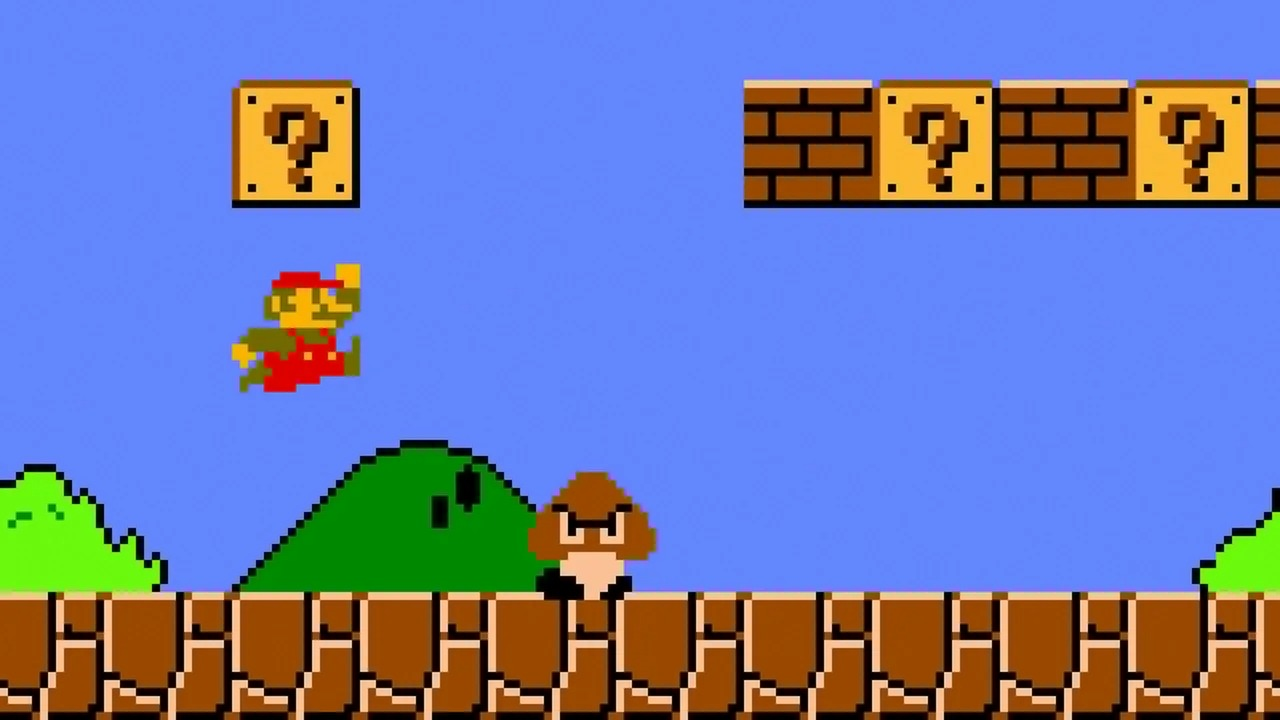
\includegraphics[width=0.8\textwidth]{images/super-mario-bros.jpg}
        \caption{Gra "Super Mario Bros" z~1986. Źródło: \cite{Mario}}
        \label{fig:SuperMarioBros}
    \end{figure}
       \begin{figure}[hpt!]
        \centering
        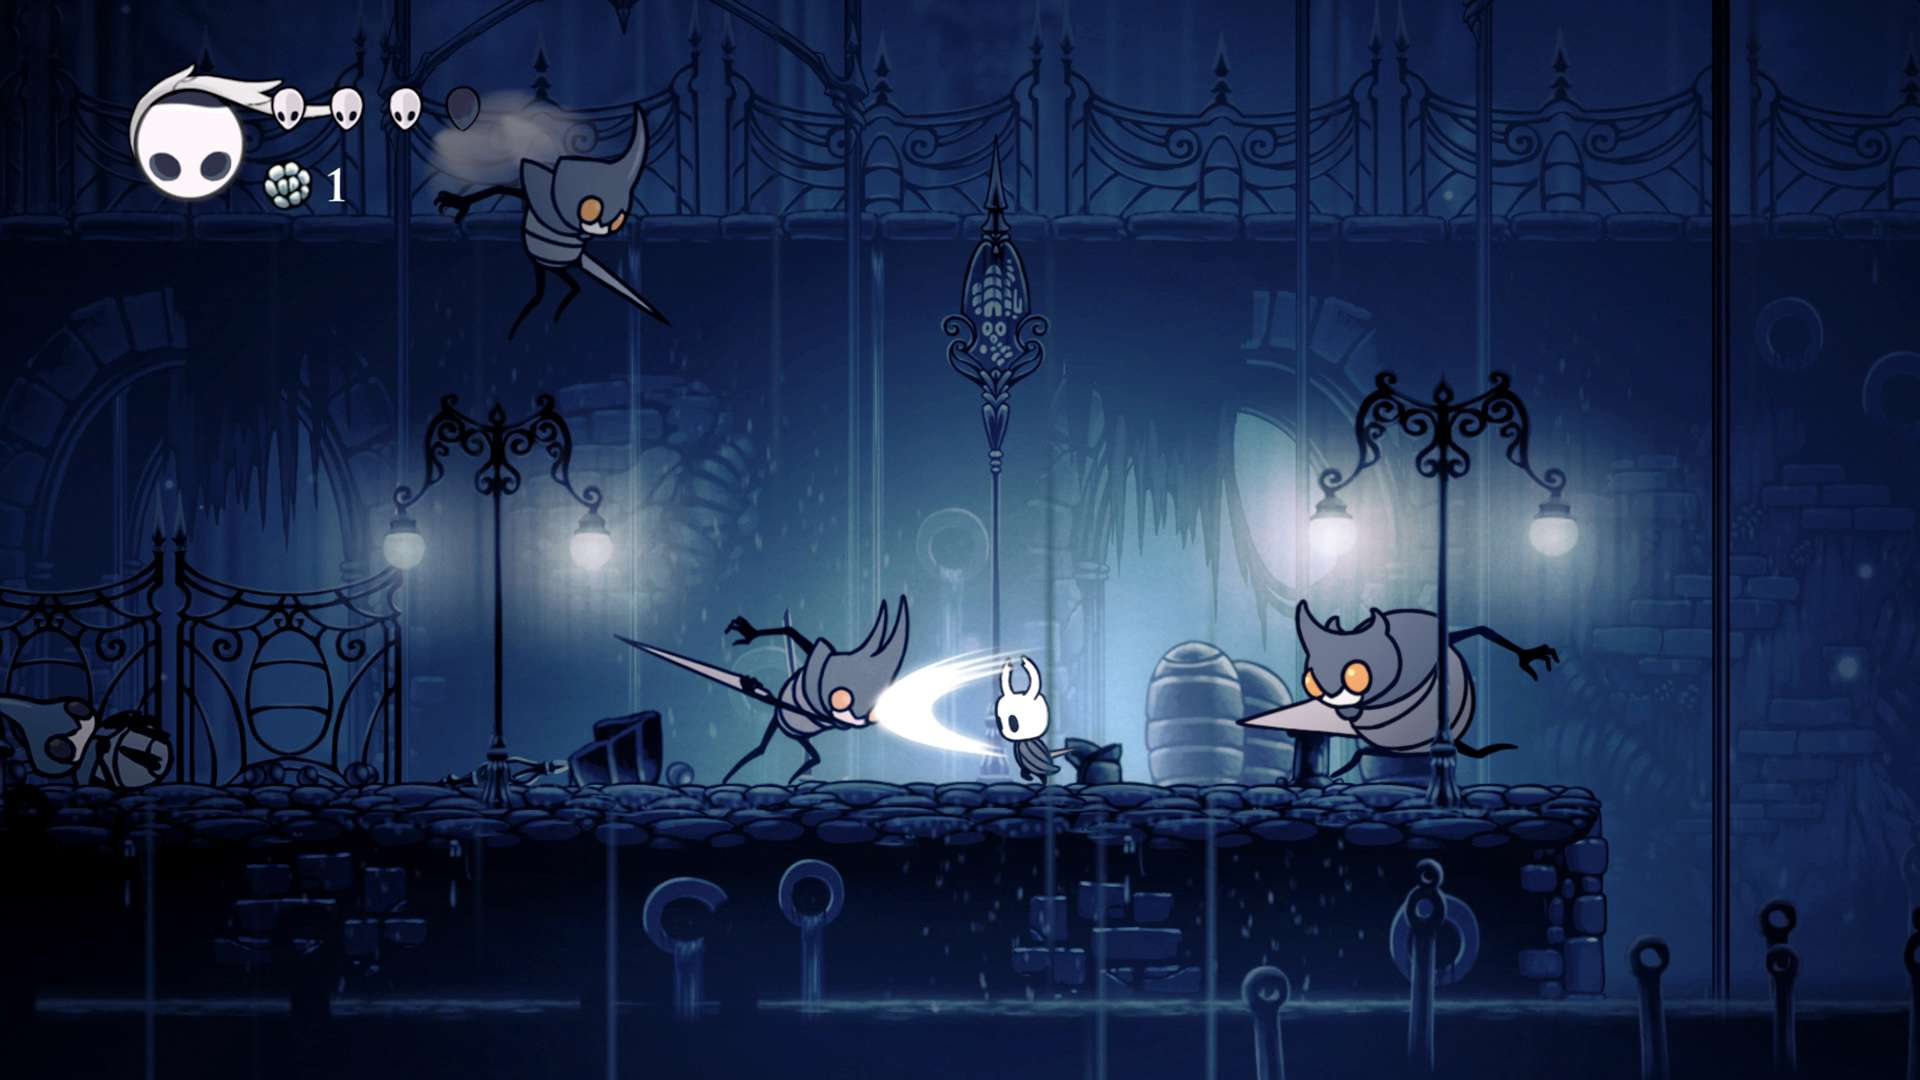
\includegraphics[width=0.8\textwidth]{images/Hollow-Knight-1-1.jpg}
        \caption{Gra "Hollow Knight" z~2017 Źródło: \cite{HollowKnight}}
        \label{fig:HollowKnight}
    \end{figure}
\newpage
\par Obecnie na rynku gier istnieje bardzo dużo takich tytułów. Są one wydawane na każdą platformę. Zazwyczaj nie wymagają one wysokiej jakości sprzętu, ponieważ najczęściej są to gry typu 2D. Idealnie nadają się one do przedstawienia różnego typu zagadnień logicznych.


\section{Tworzenie gier komputerowych}
\subsection{Zespoły tworzące gry komputerowe}
Obecnie na świecie istnieje wiele firm, które produkują gry komputerowe. W~zależności od wielkości studia skład takiego zespołu może się różnić: jedne zespoły mogą składać się z~kilku osób, inne natomiast z~kilkuset. W~procesie tworzenia gry komputerowej można wyszczególnić kilka głównych grup. Podążając za  Rafałem Nowocieniem \cite{KompendiumProd} wyróżnia się kilka ról niezbędnych do prawidłowego zrealizowania wszystkich etapów produkcji gry: zarządcze, kreatywne, artystyczne, programistyczne oraz wszystkie inne. Przyjętym na świecie standardem jest korzystanie z~angielskiego nazewnictwa stanowisk, więc tak też będą one tutaj przedstawione. Do ról zarządczych możemy zaliczyć:
\begin{itemize}
    \item \textit{Investor} - jest to indywidualna osoba lub firma, która podjęła decyzję o~finansowaniu produkcji gry. Zazwyczaj w~zamian otrzymuje ona prawa do dystrybucji gry na rynku, dzięki czemu czerpie większość zysków ze sprzedaży. W~małych zespołach czasami istnieje zjawisko polegające na tym, że wszyscy pracownicy są inwestorami - pracują oni za darmo, dzieląc się swoimi umiejętnościami podczas produkcji gry. Jeżeli ten zespół jest \textit{startupem}, osoby dzielą się umiejętnościami w~ramach \textit{opensource}.
    \item \textit{Producer} - osoba pełniąca rolę \textit{Project managera}, która jest "łącznikiem" między zespołem produkującym grę, a~inwestorem. Jej głównymi zadaniami są: planowanie budżetu, rozwiązywanie problemów, pojawiąjących się na etapie tworzenia produkcji oraz za ułatwianie komunikacji między poszczególnymi członkami zespołu.
    \item \textit{Lead programmer} - zawsze jest to osoba, która ma największe doświadczenie na stanowisku programisty. Jego zadaniem jest zarządzanie zespołem programistów oraz tworzenie dokumentacji technicznej gry.
    \item \textit{Lead designer} - jest to osoba, która odpowiada za przebieg rozgrywki, przygotowanie scenariusza gry oraz wszystkich niezbędnych w~niej mechanizmów oraz nadzorowanie pracy działu kreatywnego.
    \item \textit{Art director} - osoba, która nadzoruje tworzenie warstwy wizualnej gry.
\end{itemize}
\par Kolejną grupą funkcji są role kreatywne. Osoby pracujące w~tych zespołach odpowiadają za fabułę, wygląd poszczególnych etapów gry itp. Można tutaj zaliczyć takie stanowiska jak:
\begin{itemize}
    \item \textit{Game designer} - osoba będąca na tym stanowisku jest odpowiedzialna za projektowanie i~testowanie mechanizmów rozgrywki. W~mniejszych zespołach odpowiada ona za wszystkie poniższe pozycje w~rolach kreatywnych.
    \item \textit{Narrative designer/writer} - jest to osoba, która tworzy wszystkie elementy fabularne takie jak: opisy lokacji, opowieści, notatki czytane przez gracza oraz dialogi.
    \item \textit{Level designer} - jest to projektant poziomów gry. Jego zadaniem jest opracowanie wyglądu danej lokacji oraz postaci spotykanych przez gracza jak również poziomy trudności gry.
    \item \textit{Combat designer} - jest to osoba, która przygotowuje sekwencje walk: określa liczbę żyć przeciwników, poziomy trudności walk itp.
    \item \textit{Economy/monetisation designer} - jego zadaniem jest ustalenie ekonomicznej wartości przedmiotów w~grze. Ustala ceny towarów, tak aby w~poszczególnych poziomach gracz miał odpowiednią ilość pieniędzy.
\end{itemize}

\par Osoby, które można przypisać do ról artystycznych są odpowiedzialne za wszystkie grafiki oraz animacje w~produkcjach. Praca ta jest jedną z~najważniejszych w~całym procesie tworzenia gry, ponieważ to ich grafiki będą widoczne dla końcowych użytkowników. W~ich skład wchodzą takie stanowiska jak:
\begin{itemize}
    \item \textit{Graphic designer} - jest to osoba przygotowująca poszczególne elementy graficzne do gry. Można tę pozycję podzielić na 2 typy: graficy 2D (rysunki przedstawione są w~2 wymiarach, tzw. "płaski rysunek") oraz 3D (takie jak bryły trójwymiarowe, pojazdy i~budynki).
    \item \textit{GUI designer} - jego zadaniem jest przygotowanie interfejsu dla użytkownika, czyli: wyglądu ekranu gry, przycisków oraz ramki, dobór odpowiednich czcionek do tekstów wyświetlanych na ekranie itp.
    \item \textit{Motion designer/animator} - jego zadaniem jest zaprojektowanie wszystkich animacji w~grze, np.: realistyczne animacje chodzenia, walki lub efektów świetlnych.
    \item \textit{Cinematic designer} - do jego zadań należy projektowanie tzw. \textit{cutscen}\cite{Cutscena} - przerywników w~grze, umieszczanych w~najważniejszych momentach rozgrywki.
    \item \textit{Concept artist} - jego praca traktowana jest jako wzór dla wszystkich osób z~działu artystycznego. Jego głównym zadaniem jest przygotowanie odręcznych grafik, na podstawie których wykonywane są widzialne dla użytkownika animacje i~rysunki.
\end{itemize}

\par Role programistyczne polegają na tworzeniu kodu, który wykorzystuje wcześniej przygotowane grafiki, aby gra stała się bardziej przystępna dla użytkownika. Możemy tutaj wymienić:
\begin{itemize}
    \item \textit{Game developer} - jest to osoba, która przygotowuje kod, w~taki sposób, aby współgrał on z~grafikami i~stał się odpowiedni w~odbiorze dla gracza.
    \item \textit{Backend developer} - jest to specjalistyczna rola programistyczna. Osoba pracująca jako \textit{"backendowiec"} odpowiada za warstwę logiczną gry, gdzie dokonywane są wszystkie obliczenia.
    \item \textit{Engine programmer} - jest to osoba, która pisze bądź rozszerza zakres możliwości tzw. \textit{silników gry}, które są narzędziami usprawniającymi pisanie kodu oraz ograniczającymi liczbę linii kodu, który musiałby być tworzony dla każdej gry. 
\end{itemize}

\par Istnieją role, których nie można jednoznacznie zakwalifikować do żadnych z~wyżej wymienionych kategorii. Osoby te często wykonują zadania z~wyżej wymienionych stanowisk oraz do ich obowiązków należy popularyzacja gry. Możemy tutaj zauważyć takie stanowiska jak: 
\begin{itemize}
    \item \textit{Sound/music designer} - osoba zatrudniona na tym stanowisku odpowiedzialna jest za dźwięki, które możemy usłyszeć podczas rozgrywki.
    \item \textit{Tester} - jedno z~cięższych stanowisk podczas produkcji gier. Osoba ta szuka błędów w~grze i~zgłasza je osobom odpowiedzialnym za poszczególne komponenty produkcji.
    \item \textit{Marketing manager} - jego zadaniem jest promowanie gry na rynku oraz współpraca z~mediami.
    \item \textit{Community manager} - stosunkowo nowe stanowisko podczas produkcji gier. Osoba zatrudniona jako community manager odpowiedzialna jest za utrzymywanie zainteresowania użytkowników daną produkcją, udziela odpowiedzi na wszystkie pytania graczy związane z~nadchodzącym tytułem.
    \item \textit{Customer service} - jego praca rozpoczyna się po premierze gry. Jest on odpowiedzialny za pomoc użytkownikom w~problemach technicznych związanych z~daną produkcją.
    \item \textit{ASO manager} - osoba, której zadaniem jest pozycjonowanie gry w~najpopularniejszych serwisach sprzedażowych.
    \item \textit{Translator} - osoba zatrudniona jako translator odpowiedzialna jest za tłumaczenie tekstów - zarówno pisanych jak i~mówionych - aby gra była dostępna dla szerzej grupy potencjalnych konsumentów.
    \item \textit{Porting team} - jest to jedno z~najtrudniejszych zadań podczas całego etapu tworzenia gier. Osoby pracujące w~tym zespole zajmują się przenoszeniem gry na inne dostępne na rynku platformy, co wymaga poważnych zmian w~kodzie i~grafice. Zazwyczaj w~skład takiego zespołu wchodzą najbardziej doświadczeni programiści i~graficy.
\end{itemize}
\subsection{Etapy tworzenia gier komputerowych}
\par Proces powstawania gry komputerowej jest bardzo czasochłonny. Aby dana produkcja odniosła sukces, osoby odpowiedzialne za projekt muszą się ciągle rozwijać, tak aby podążać za najnowszymi trendami na rynku. W~obecnych czasach na świecie jest bardzo dużo osób, które grają w~takie produkcje. Większość z~nich nie jest świadoma tego ile czasu zajmuje powstanie gry. Cały proces tworzenia produkcji bardzo trafnie opisano w~\cite{KompendiumProd}, został on podzielony na trzy fazy:
\begin{enumerate}
    \item Faza preprodukcyjna,
    \item Faza produkcyjna,
    \item Faza postprodukcyjna.
\end{enumerate}
\subsubsection{Faza Preprodukcyjna}
\par Jest to czysto teoretyczna faza w~całym etapie tworzenia gier komputerowych. Podczas jej trwania przygotowywane zostają wszystkie informacje oraz dokumenty, które będą przydatne do otrzymania efektu końcowego - publikacji gry.

\par Pierwszym elementem tej fazy jest opracowanie \textit{Koncepcji gry}, czyli tego czym produkcja ma być. Określony zostaje tutaj typ gry np.: gra platformowa, rodzaj (2D bądź 3D) oraz założenia projektowe, którymi są informacje o~graczu, jego podstawowe zadania itp.

\par Kolejnym etapem jest utworzenie \textit{Głównego Dokumentu Koncepcyjnego}, czyli \textit{GDD}. W~tym dokumencie zawarte są szczegółowe informacje dotyczące danej gry: tematyka, grupa docelowa graczy (określany jest typ graczy, którzy mogą być zainteresowani produkcją), przedmioty dostępne w~grze, szczegóły opisujące przeciwników. Bardzo ważnym elementem tego dokumentu są grafiki koncepcyjne, które przedstawiają propozycje wyglądu poszczególnych obiektów ukazanych w~produkcji. Projektant gry opracowując \textit{GDD} konsultuje go z~inwestorem, głównym programistą oraz dyrektorem artystycznym w~celu przedstawienia i~uzgodnienia wizji danej produkcji.
\par Na podstawie wyżej opisanego \textit{GDD} główny programista tworzy \textit{Dokument Techniczny Gry}, czyli \textit{GTD}. Zawarte są w~nim wymagania sprzętowe, informacje odnośnie wykorzystywanego silnika gry oraz inne przydatne informacje techniczne. Dokument ten zawiera również harmonogram produkcji poszczególnych elementów gry. Równocześnie z~\textit{GDD} tworzony jest \textit{Dokument Poziomów Gry}, czyli \textit{LDD}. Zawiera on w~sobie informacje o~poszczególnych poziomach, opisy kampanii oraz zadania dla gracza. Obydwa te dokumenty podlegają ciągłym zmianom podczas kolejnych etapów tworzenia gry.
\par Podczas Fazy Preprodukcyjnej tworzone są również pomocnicze dokumenty, inne niż te wyżej wymienione, są to m.in.: plan produkcji oraz budżetowy, lista dźwięków, dokumenty fabularne, plany marketingowe i~wiele innych.

\subsubsection{Faza Produkcyjna}
\par Podczas trwania \textit{fazy produkcyjnej} wykorzystywane są materiały opracowane podczas poprzedniego etapu. Na początku zostaje przygotowany prototyp, który jest pierwszą, bardzo okrojoną wersją gry, mającą na celu przedstawienie działania i~wyglądu końcowej produkcji. Sprawdzane są tutaj również założenia początkowe z~fazy preprodukcyjnej, czy zostały one zrealizowane w~tworzonej grze. Kolejnym prototypem jaki zostaje przygotowany jest \textit{Vertical Slice}. W~przeciwieństwie do MVP, który służy zastosowaniom zespołu produkcyjnego, \textit{VS} ma za zadanie pokazać odbiorcom jak będzie wyglądał efekt końcowy, ma ich zaciekawić, aby wyczekiwali oni publikacji gry.

\par Ostatnim etapem tej fazy jest przygotowanie tzw. \textit{beta buildu}. Jest to dużo bardziej rozbudowana wersja gry, z~którą odbiorcy mieli styczność podczas prezentowania MVP i~VS. Zawiera on w~sobie wszystkie zaplanowane elementy wersji końcowej, jednakże jeszcze nie do końca działające poprawnie. Służy on przede wszystkim do testowania funkcjonalności oraz do znajdywania różnych błędów, tak aby użytkownik mógł cieszyć się w~pełni działającą grą. Bardzo często zauważa się, że firmy działają na zasadzie \textit{Open Beta Testów}. Oznacza to, że udostępniają oni swój produkt graczom, a~oni grając sprawdzają poprawność działania.

\subsubsection{Faza Postprodukcyjna}
\par Ostatnia faza produkcji gry polega na opublikowaniu gry na rynku, oraz poprawianiu niezauważonych wcześniej błędów. Na tym etapie udostępniane są również dodatkowe materiały związane z~tytułem, np.: ubrania z~logiem gry, soundtracki, czyli ścieżki dźwiękowe użyte w~rozgrywce i~wiele innych.

\par Pierwszym krokiem jest wybranie odpowiedniego kandydata wersji gry do publikacji, tzw. \textit{Release Candidate}. Decyzja o~wyborze buildu końcowego podejmowana jest zazwyczaj przez \textit{Project managera} oraz \textit{Investora} bądź \textit{Wydawcę}. Aby gra mogła przejść z~fazy \textit{Beta testów} do \textit{RC}, musi ona przejść przez \textit{Testy akceptacyjne}\cite{TestyAkceptacyjne}, które pomagają określić czy dana produkcja jest gotowa do publikacji. Sprawdza się tutaj między innymi zachowanie gry z~określoną wcześniej specyfikacją itp.

\par Gdy \textit{RC} przejdzie wszystkie niezbędne procedury, podejmowana jest decyzja o~publikacji. Od wcześniej zbudowanego tła przez osoby zajmujące się marketingiem i~promowaniem produkcji zależy powodzenie sprzedaży produktu. Producenci bardzo często korzystają w~celu zwiększenia sprzedaży swojego tytułu z~różnych pośredników, takich jak na przykład Steam\cite{Steam}, który jest największym dystrybutorem gier na rynku. Przedsiębiorstwa programistyczne bardzo często decydują się na samodzielne wydanie gry. Bardzo ważną rolę odgrywają tutaj serwisy społecznościowe, na których prowadzona jest kampania marketingowa.

\par Bardzo często zdarza się, że po wydaniu danej gry firmy oferują wsparcie dla klienta. Dzieje się to, ponieważ podczas testowania nie da się znaleźć wszystkich błędów działania danego tytułu. Dzięki temu, użytkownik który zauważy problem może zgłosić się do osoby wykwalifikowanej która rozwiąże problem tak, aby z~czasem gra stała się pozbawiona błędów i~zapewniała rozrywkę dla osób, które zdecydują się ją zakupić.


%############################################################################################
%############################################################################################
%-----------               Rozdział 2. Fabuła Gry "Tree of Life"                 -----------# 
%############################################################################################
%############################################################################################

\chapter{Fabuła gry "Tree of life"}
\par Rozdział skupia się na przedstawieniu fabuły gry - ukazana zostanie historia głównego bohatera. Opisane również zostaną pomysły, których nie udało się zrealizować podczas tworzenia tej produkcji oraz potencjalne możliwe scenariusze rozwoju tego tytułu.

\section{Pomysły zrealizowane}

\subsection{Przeszłość}
\par W~grze \textit{Tree of Life} gracz wciela się w~postać legendarnego wikinga o~imieniu \textit{Björn Żelaznoboki}, który jest synem \textit{Ragnara Lothbroka} pochodzącego od nordyckiego boga \textit{Odyna} oraz wojowniczej królowej \textit{Lagerthy}. Swój przydomek zdobył podczas jednej z~wypraw, gdzie wyróżnił się wielką odwagą i~determinacją w~pokonaniu podbijanego przez wikingów ludu. Tak jak ojciec jest on inteligentny i~zdeterminowany: pragnął przygód oraz poznania innych kultur i~narodów. Po tragicznej śmierci Ragnara został on królem miasta - państwa \textit{Kattegat}. Z~jednego ze swoich nieudanych małżeństw miał córkę \textit{Siggy}.


\subsection{Teraźniejszość}
\subsubsection{Poszukiwanie lekarstwa}
\par Właściwa historia przedstawiona w~grze rozpoczyna się w~momencie odkrycia, że córka Björna jest ciężko chora i~nie ma szans na przeżycie. Bohater nie załamuje się i~postanawia wyruszyć na wyprawę do odległych krain, aby znaleźć dla niej lekarstwo. Podczas poszukiwań w~pewnym kraju jeden z~wikingów trafił na wędrowca. Włóczęga opowiedział mu o~bardzo niebezpiecznym terytorium, w~którym rośnie drzewo łączące ze sobą wszystkie światy - \textit{Yggdrasil}. Według dawnych podań osoba, która dostanie się na szczyt tego starodrzewa otrzyma napój leczący wszystkie choroby. 

\par Wojownik ucieszył się z~tej informacji i~zabrał wędrowca ze sobą na spotkanie z~królem. Podróżnik opowiedział ze szczegółami całą historię tej krainy i~przestrzegał, żeby Björn nie udawał się tam, ponieważ czeka go niechybna śmierć. Miłość bohatera do córki jest jednak tak ogromna, że zamierza on poświęcić własne życie dla niej: nie przejmuje się tym, że cała jego kompania może nie wrócić do domów. Znając ryzyko dał możliwość podjęcia decyzji swoim wikingom zdecydować czy chcą płynąć z~nim czy wolą wrócić do domów. Większość z~nich wybrała towarzyszenie swojemu \textit{jarlowi} w~wyprawie, ponieważ kochali go. Dzięki niemu ich wioska stała się najpotężniejszą osadą w~całej Norwegii, to on zapewnił im dobrobyt i~przyszłość. 

\par Wraz z~wojownikami, którzy zdecydowali się wyruszyć z~królem, Björn rozpoczął przygotowania do wyprawy. Nie wiedząc, jak daleka podróż ich czeka, wyładowali oni drakkary do granic możliwości prowiantem, wodą oraz różnego rodzaju bronią, które zakupili w~pobliskiej wiosce. Na morzu kompania spędziła dużo tygodni. Ich zapasy były na wykończeniu. Pewnego dnia, gdy byli na otwartym morzu, zastał ich sztorm: drakkary zostały oddzielone od siebie, część została zniszczona przez żywioł. Jednym ze zniszczonych statków była łódź, którą płynął Björn. Krew nordyckiego boga \textit{Odyna} płynąca w~żyłach nordyckiego króla sprawiła, że tylko on przetrwał ten kataklizm. Po wielu dniach dryfowania na szczątkach drakkaru na morzu trafił on na dziwnie wyglądającą wyspę.

\subsubsection{Mroczna Kraina}
\paragraph{Plaża}\hfill \break
\par Ranny i~wycieńczony wiking widząc, że miejsce w~którym się znajduje nie sprzyja ludziom, zaczął szukać schronienia. Znalazł zaciszną jaskinię, w~której postanowił odpocząć. Po kilku dniach spędzonych w~grocie Björn postanowił poszukać jedzenia i~jakiejkolwiek osady. Podczas wędrówki został on jednak złapany przez dziwnie wyglądające stwory - \textit{Draugry}\cite{Draugr}. Są to najbardziej mroczne stworzenia pochodzące z~pierwotnych skandynawskich legend. Potwory te przypominały z~wyglądu ludzi - wikingów, ale w~przeciwieństwie do króla Kattegat postacie te nie żyły. Demony te są zmarłymi wojownikami, które za sprawą czarnej magii zostały wskrzeszone. Uosabiają one lęk wikingów przed zmarłymi. W~postaci tych potworów zło ukazywało się przez nienawiść do wszystkiego co żyje. Żelaznoboki został zabrany do dziwnie wyglądającej cytadeli - siedziby demonów, tam został zamknięty w~celi.

\paragraph{CONDEMNED CITADEL}\hfill \break
\par Po kilku dniach przebywania w~zamknięciu Björn został wezwany przed oblicze władcy Draugrów - \textit{Jormungand} - który był bogiem, przeciwnikiem Thora, boga piorunów, w~postaci gigantycznego węża. Król wyspy chce, aby wiking stał się jego sługą, na co ten nie chce się zgodzić. Z~tego powodu zostaje zamknięty w~więzieniu i~torturowany. Pewnego dnia po męczarniach znajduje w~celi mapę i~list mówiący o~\textit{Drzewie Życia}, o~którym opowiadał mu wcześniej napotkany podróżnik. Żelaznoboki uradował się, ponieważ dotarł do miejsca, gdzie chciał się znaleźć, aby uratować swoją córkę. 

\par Kolejnego dnia, gdy znowu został zabrany na tortury, ukradł narzędzie, które będzie mu służyć jako wytrych do otwarcia drzwi celi. Bohater odkrył w~sobie nowe pokłady siły i~teraz, każdego dnia po męczarniach żłobił ukradzione narzędzie, tak aby mógł on otworzyć zamek i~wydostać się na wolność. Znanemu ze swojej determinacji Björnowi zajęło to kilka wieczorów. Podczas jednej z~pracowitych nocy, znalazł w~pobliżu drzwi na ścianie dziwną liczbę, jednak zignorował ją - twierdząc, że jest to pozostałość po poprzednim więźniu.

\par Pewnego wieczoru po dniu pełnym tortur postanowił wcielić swój plan w~życie. Przed sobą miał mechanizm (zob. rysunek \ref{ZamekCeli}) - zamek do drzwi, który można było odblokować ustawiając w~odpowiedniej kolejności piny.

\begin{figure}[hpt!]
        \centering
        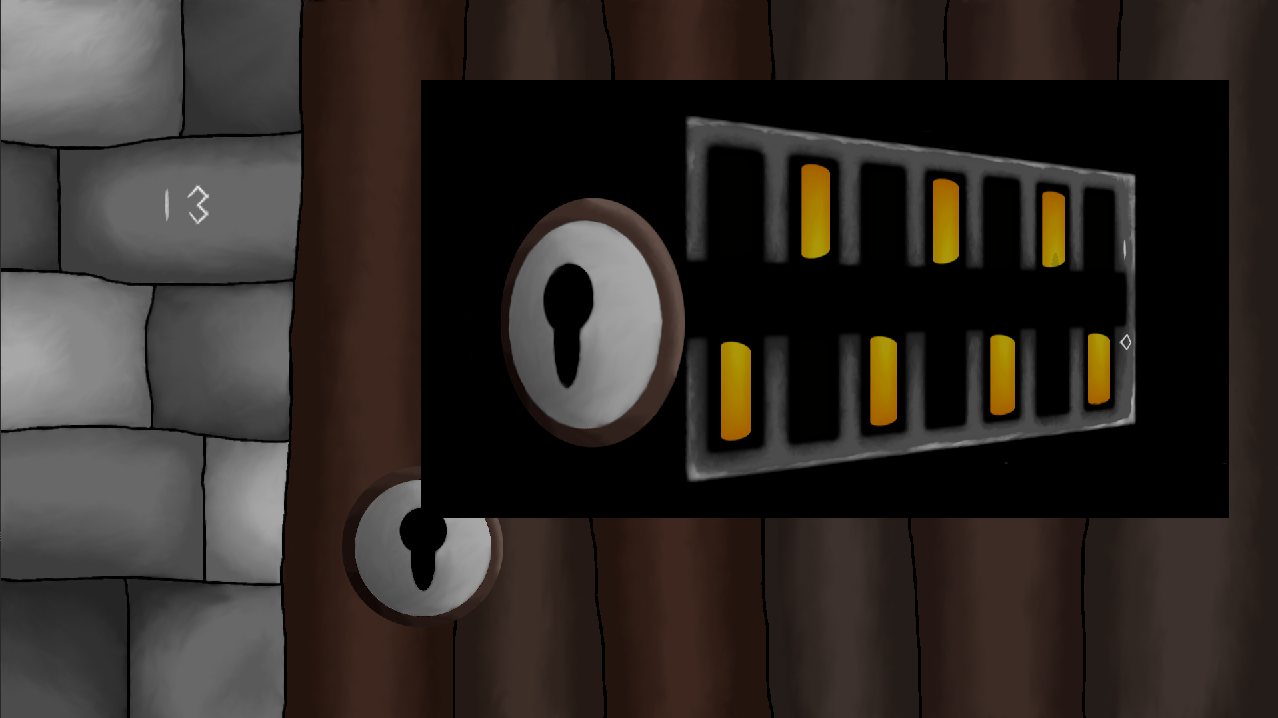
\includegraphics[width=0.8\textwidth]{poziomy/binaryconvert.png}
        \caption{Wygląd mechanizmu zamka}
        \label{ZamekCeli}
    \end{figure}
\par Zamek składa się z~7 pinów. Król wikingów próbował różnych sposobów, aby otworzyć drzwi jednak mu się to nie udało. Przypomniał sobie o~liczbie wyżłobionej na ścianie w~okolicy drzwi. Postanowił ją wykorzystać.
Okazało się, że liczba ta niewiele pomaga w~próbie otwarcia mechanizmu zamka. Zmęczony i~poirytowany Björn zaczął czytać jeszcze raz znaleziony list, w~którym odnalazł wskazówkę (zob. rysunek \ref{Helper}) jak przekształcić znalezioną liczbę w~ciąg cyfr, służący do otwarcia drzwi. 

\begin{figure}[hpt!]
        \centering
        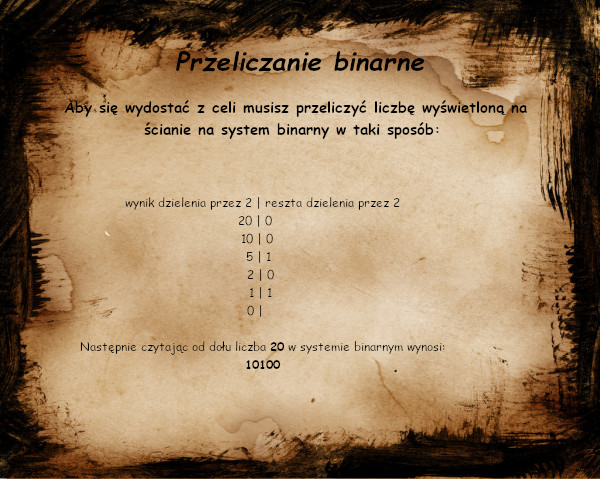
\includegraphics[width=0.8\textwidth]{podpowiedzi/helper_image.png}
        \caption{Wygląd podpowiedzi dla gracza do pierwszego poziomu}
        \label{Helper}
    \end{figure}

\par Aby wydostać się z~więzienia gracz musi przekształcić wyrytą liczbę na ciąg cyfr w~systemie binarnym. Położenie poszczególnych pinów odzwierciedla '0' bądź '1'. Gdy użytkownikowi wcielającemu się w~postać króla wikingów uda się rozwiązać zagadkę, drzwi się otwierają. W~korytarzu Björn znajduje topór, który będzie mu służył do obrony przed napotkanymi przeciwnikami.

\paragraph{SVARTAL}\hfill \break

\par Szczęśliwie, królowi Kattegat udaje się wydostać z~cytadeli, w~której był więziony. Trafia on do królestwa \textit{Mrocznych elfów} (zob. rysunek \ref{SvartalPlatform}). Są to bardzo niebezpieczne istoty zamieszkujące ciemne miejsca, charakteryzujące się posiadaniem czerwonych oczu oraz szarym odcieniem skóry, co odróżnia je od innych elfów. Żyją one bezpieczne w~podziemiach twierdzy\textit{Jormunganda}. 

\begin{figure}[hpt!]
        \centering
        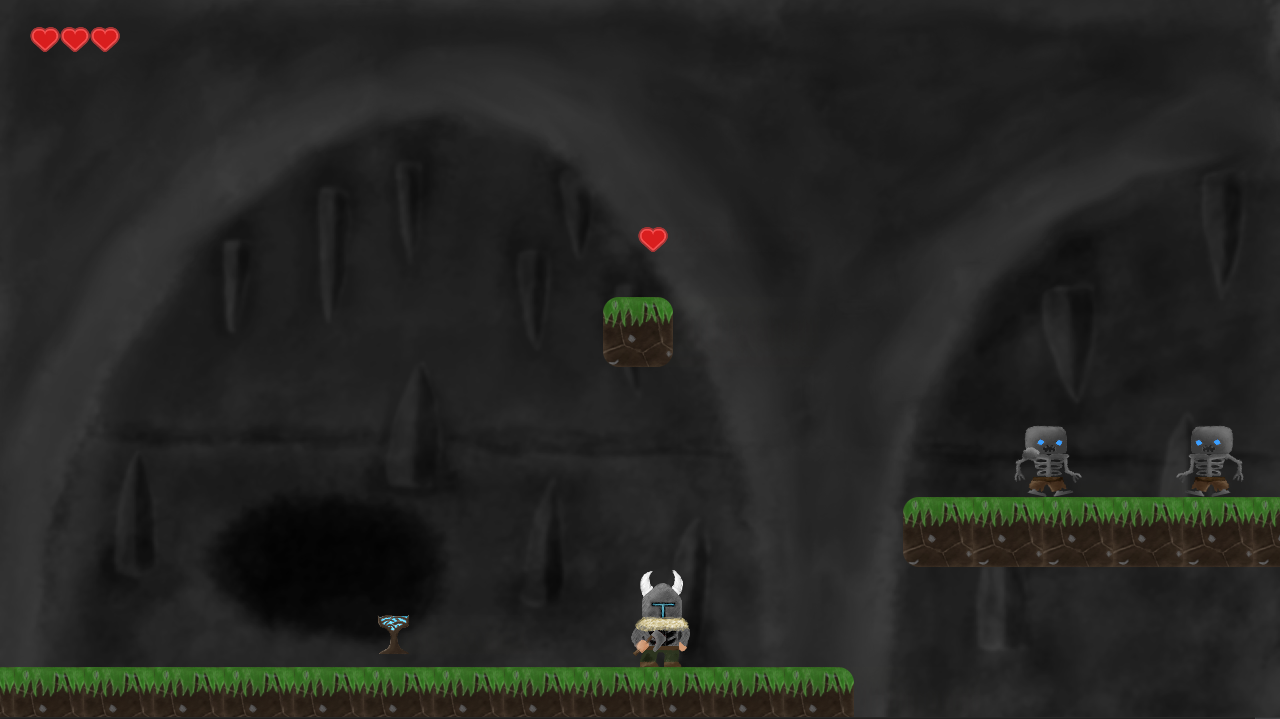
\includegraphics[width=0.8\textwidth]{poziomy/svartal.png}
        \caption{Przykładowy wygląd poziomu w~lokacji "SVARTAL"}
        \label{SvartalPlatform}
    \end{figure}
\newpage
\par Björn musi się wydostać z~tego królestwa. Aby tego dokonać musi skakać po półkach skalnych, na których może napotkać wrogo nastawione do siebie elfy, które mogą przejawiać jeden z~trzech stanów:
\begin{itemize}
    \item Zdziwienie - postacie te krążą tylko po platformie, nie umieją strzelać, zazwyczaj można je unieszkodliwić jednym bądź dwoma strzałami z~łuku
    \item Zdenerwowanie - osobniki te potrafią strzelać, w~porównaniu do opisanych wyżej gracz będzie potrzebował oddać większą ilość strzałów, aby je unieszkodliwić
    \item Rozwścieczenie - jednostki te bardzo szybko oddają swoje strzały, posiadają najczęściej dużą "ilość" życia, gracz musi się natrudzić, aby je pokonać
\end{itemize}

\par Na swojej drodze gracz może zbierać dodatkowe życie oraz wskazówkę (zob. rysunek \ref{BubbleSortHelper}), która pomoże mu pokonać następną łamigłówkę, aby przejść do kolejnej lokalizacji. 

\begin{figure}[hpt!]
        \centering
        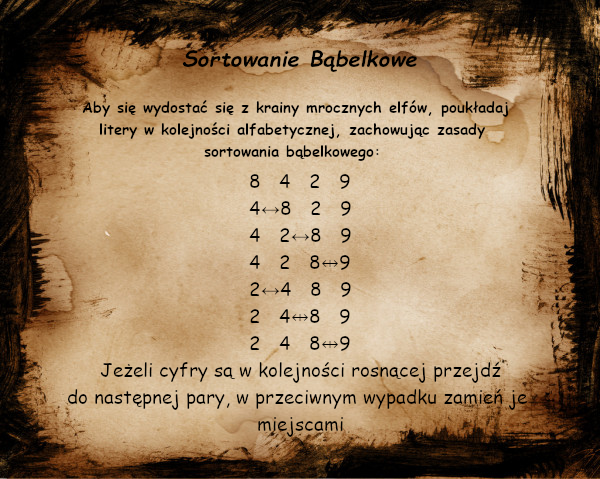
\includegraphics[width=0.8\textwidth]{podpowiedzi/helper_bubble_sort.png}
        \caption{Przykładowa podpowiedź do poziomu Bubble Sort}
        \label{BubbleSortHelper}
    \end{figure}

\par Po dotarciu do drzwi, król Kattegat musi je otworzyć układając cyfry w~odpowiedniej kolejności (zob. rysunek \ref{BubbleSort}). Mroczne elfy chcąc złapać postaci, które dostają się do ich królestwa, oraz przewidując, że strażnicy będący na skalnych półkach mogą sobie nie poradzić z~intruzem, stworzyły mechanizm blokujący drzwi, który znają tylko one. Björn podczas swojej wędrówki poprzez tę krainę może znaleźć instrukcję, opisującą w~jaki sposób może otworzyć drzwi. W~przeciwnym wypadku będzie musiał próbować odgadnąć algorytm rozwiązujący tę sekwencję.

\begin{figure}[hpt!]
        \centering
        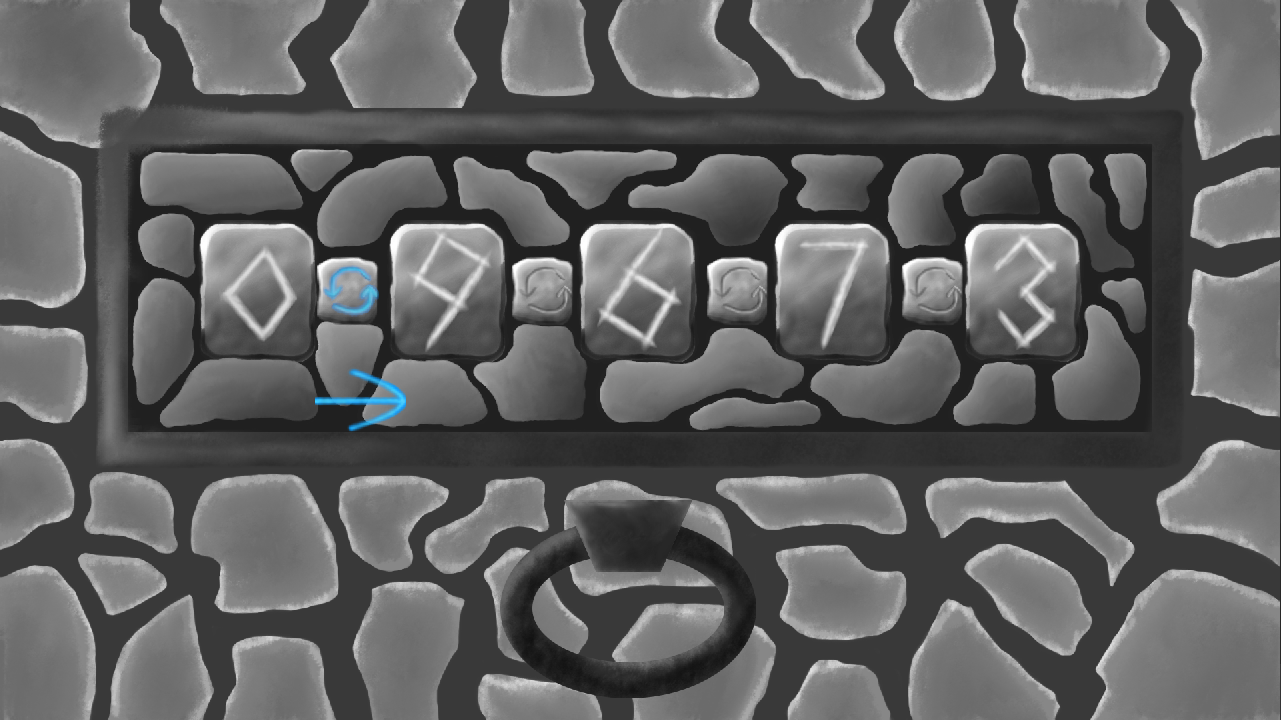
\includegraphics[width=0.8\textwidth]{poziomy/bubble.png}
        \caption{Wygląd mechanizmu wyjścia z~krainy elfów}
        \label{BubbleSort}
    \end{figure}
\newpage

\paragraph{ANCIENT FOREST}\hfill \break

\par Po wydostaniu się z~królestwa mrocznych elfów główny bohater trafia do starożytnego lasu (zob. rysunek \ref{ForestPlatform}). Na swojej drodze spotyka wysłane na poszukiwania przez \textit{Jormunganda} Draugry. Tym razem nie mają one zamiaru złapać króla Kattegat - chcą go zabić, aby nie osiągnął on celu swojej podróży - \textit{Drzewa Życia}.

\begin{figure}[hpt!]
        \centering
        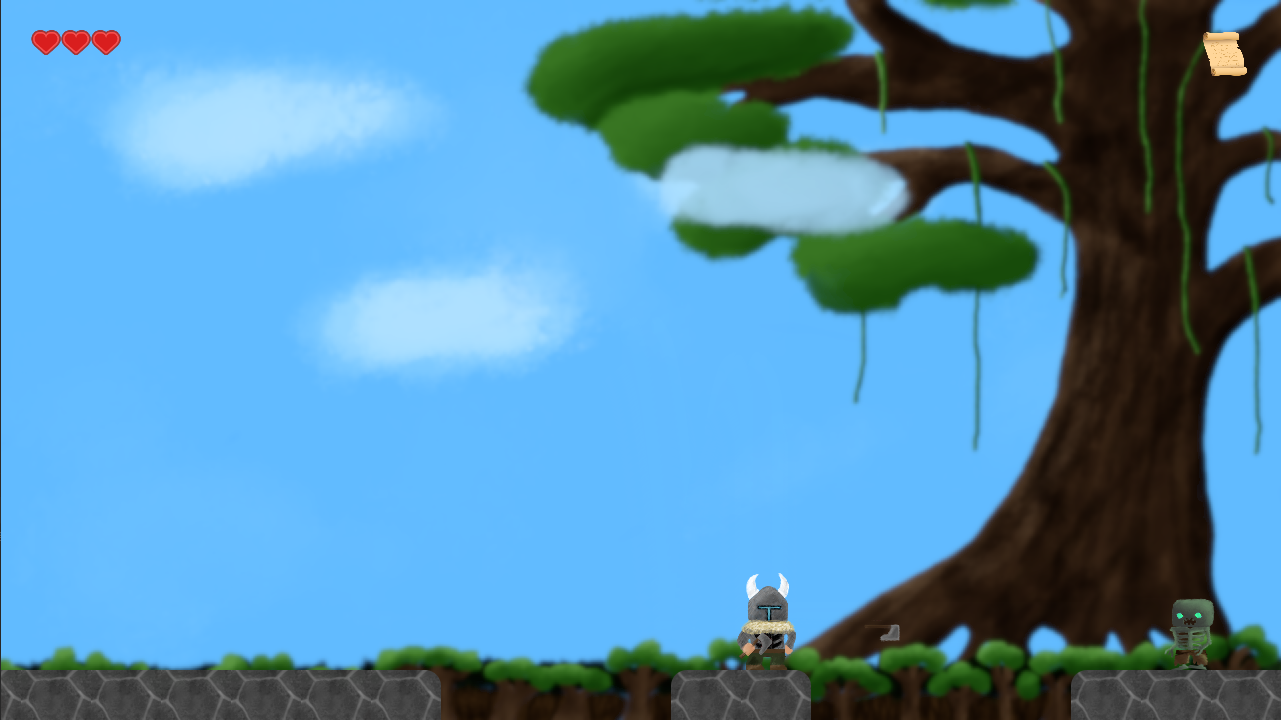
\includegraphics[width=0.8\textwidth]{poziomy/ancientforest.png}
        \caption{Przykładowy wygląd poziomu w~lokacji "ANCIENT FOREST"}
        \label{ForestPlatform}
    \end{figure}

\par Podobnie jak w~królestwie mrocznych elfów, Björn musi skacząc po platformach, pokonać przeciwników oraz znaleźć wskazówkę. Tym razem jego celem nie jest wydostanie się z~królestwa, chce on dostać się do drzewa, aby zdobyć lek dla swojej córki. Lokalizacja, w~której się znajduje jest nieprzewidywalna i~pełna dziwnych mocy. Na każdym kroku na gracza czeka niebezpieczeństwo w~postaci przeciwników bądź dziwnych przeszkód.

\par Mijając platformy u podnóża starodrzewa, oczom gracza ukazuje się ogromna brama. Aby przez nią przejść trzeba zaszyfrować słowo w~odpowiedni sposób. Żelaznoboki musi łapać klocki i~przeciągać je w~przeznaczone do tego miejsce, tak aby powstał \textit{szyfrogram}, czyli ciąg znaków, który po odpowiednim przekształceniu da użytkownikowi tekst jawny, otrzymany na początku. Aby rozwiązać łamigłówkę gracz musi znać zasadę szyfrowania według \textit{szyfru PlayFair} \ref{PlayfairMechanism}. Król Kattegat musi się śpieszyć, ponieważ w~każdej chwili mogą na niego napaść Draugry bądź Mroczne Elfy.\hfill \break

\begin{figure}[hpt!]
        \centering
        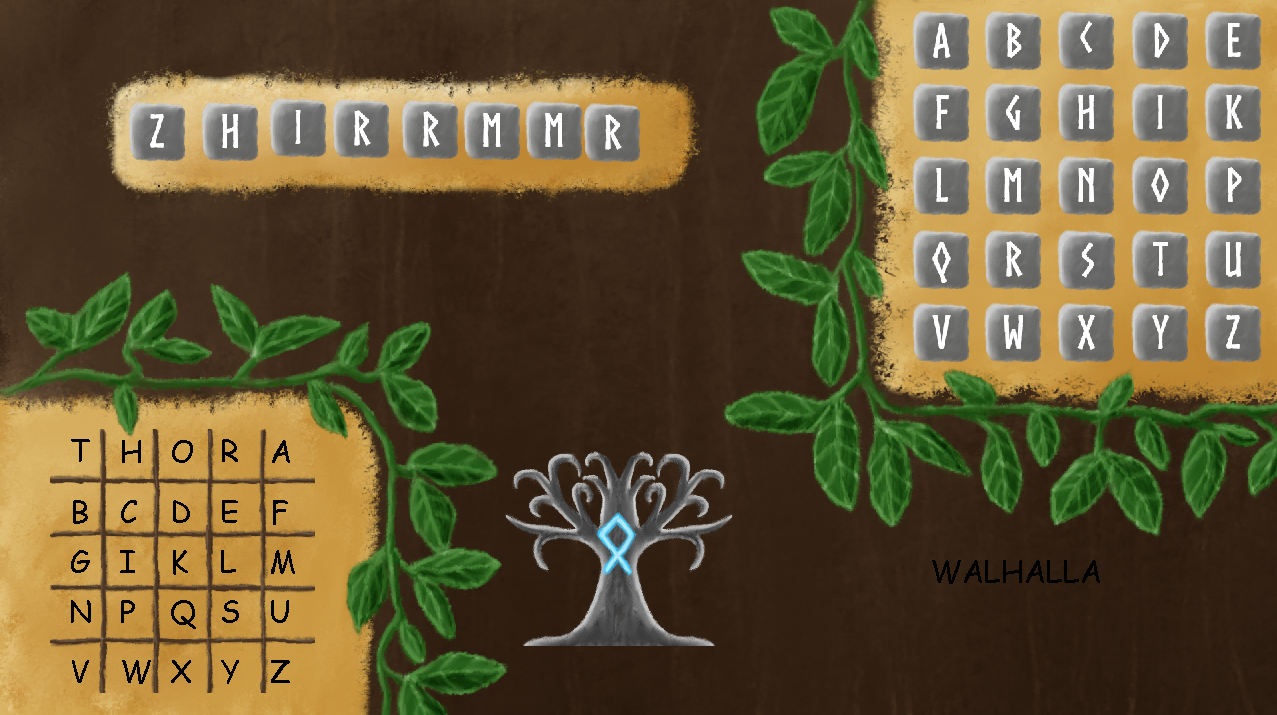
\includegraphics[width=0.8\textwidth]{poziomy/playfair.png}
        \caption{Przykładowy wygląd mechanizmu bramy}
        \label{PlayfairMechanism}
    \end{figure}
\newpage
\par Podczas trwania "części platformowej" poziomu król wikingów może znaleźć wskazówkę (zob. rysunek \ref{PlayfairHelper}), która może mu pomóc w~rozwiązaniu łamigłówki. Jeżeli jej nie zabierze, będzie musiał próbując różnych kombinacji odnaleźć 
odpowiedni ciąg znaków umożliwiający dostanie się do \textit{Yggdrasilu}.

\begin{figure}[hpt!]
        \centering
        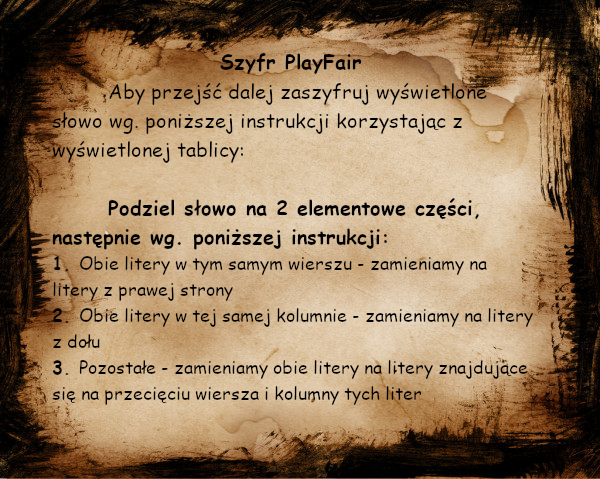
\includegraphics[width=0.8\textwidth]{podpowiedzi/playfair_helper.png}
        \caption{Przykładowa podpowiedź do poziomu PlayFair}
        \label{PlayfairHelper}
    \end{figure}
\newpage
\paragraph{Tree of Life}\hfill \break

\par Ostatnim wyzwaniem dla Björna jest przejście po odpowiednich gałęziach \textit{Drzewa Życia} (zob. rysunek \ref{TreeOfLife}). Musi on wykorzystać ciąg liter użyty do otwarcia bramy tak, aby skacząc po odpowiednich platformach dostał się do upragnionego lekarstwa dla swojej córki (zob. rysunek \ref{TreeOfLifeHelper}). Tutaj nie czekają już na niego przeciwnicy, ponieważ wszystkie złe istoty boją się energii, która promieniuje od starodrzewa. 

\begin{figure}[hpt!]
        \centering
        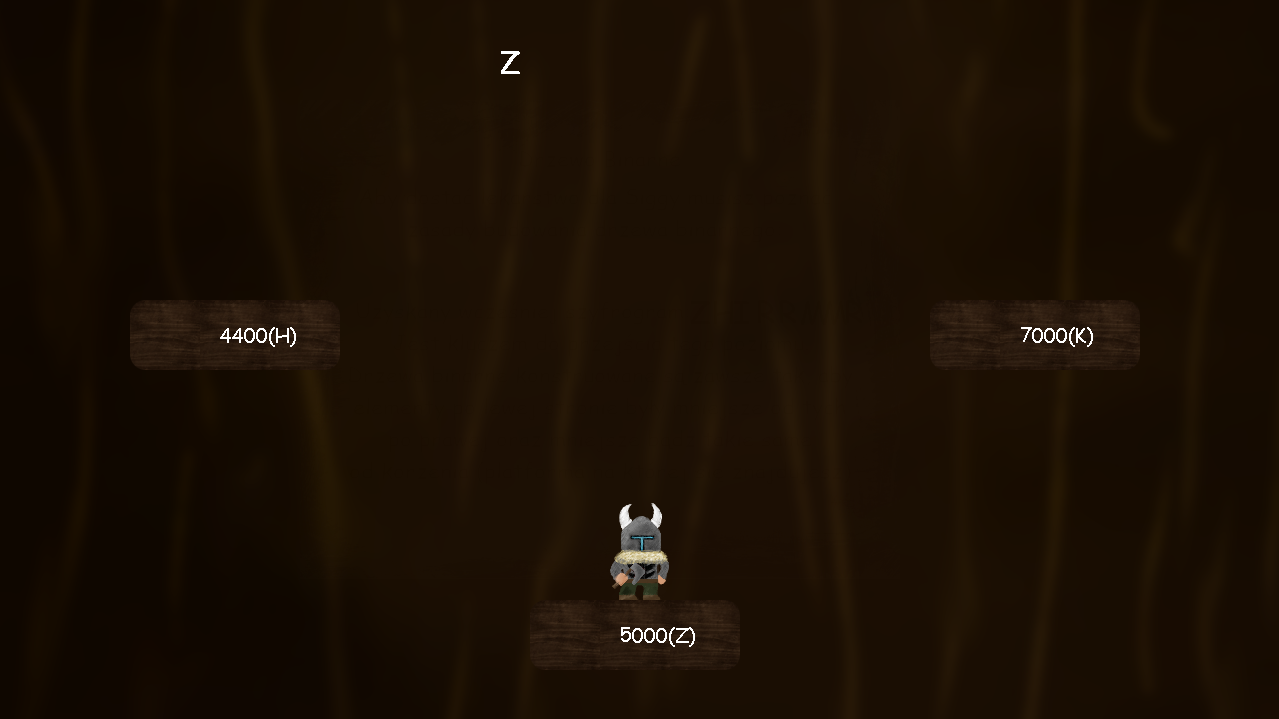
\includegraphics[width=0.75\textwidth]{poziomy/binarytree.png}
        \caption{Przykładowy wygląd gałęzi w~lokacji "Tree Of Life"}
        \label{TreeOfLife}
    \end{figure}
    
\begin{figure}[hpt!]
        \centering
        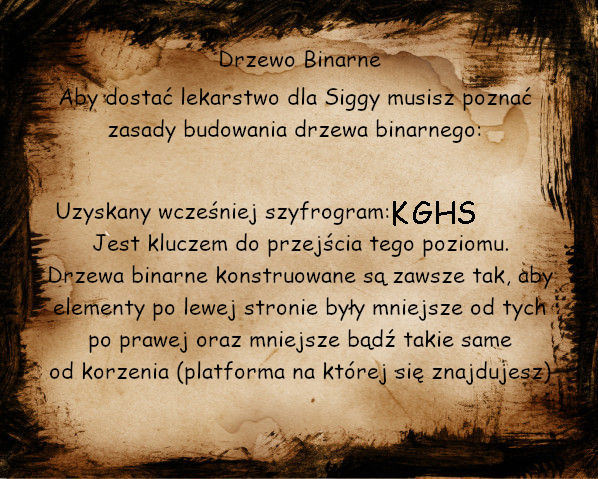
\includegraphics[width=0.75\textwidth]{podpowiedzi/binarytreehelp.png}
        \caption{Przykładowy wygląd podpowiedzi w poziomie Tree Of Life}
        \label{TreeOfLifeHelper}
    \end{figure}
    \newpage
\par Na każdej gałęzi jest znak z~literą, jaką ta odrośl reprezentuje. Po prawidłowym przejściu po odpowiedniej ścieżce Björn dostaje w~swoje ręce lekarstwo, dzięki któremu może uratować życie \textit{Siggy}. Natomiast, jeżeli gracz w~trakcie pokonywania poziomu pomyli się i~skoczy na złą gałąź, spadnie na ziemię i~będzie musiał rozpocząć swoją przygodę z~pokonywaniem drzewa od początku.
    
\section{Pomysły niezrealizowane}
\par W~fazie preprodukcyjnej pomysłem było utworzenie większej ilości lokalizacji, w~której gracz mógłby się poruszać oraz dodanie bardziej zróżnicowanych przeciwników, jak również schematów, dzięki którym inaczej odbywałyby się walki z~napotkanymi podczas rozgrywki postaciami. Przedstawione tutaj lokalizacje są wybranymi z~wymyślonych wcześniej, ponieważ gra która zawierałaby w~sobie to wszystko co zostanie poniżej opisane byłaby niedopracowana, pełna różnych błędów. Podczas tworzenia \textit{Głównego Dokumentu Koncepcyjnego} przewidziane były następujące lokalizacje:
\begin{enumerate}
    \item \textit{CONDEMNED CITADEL} - lokacja użyta w~finalnej wersji gry, w~zamyśle miała być podzielona na kilka mniejszych:
    \begin{itemize}
        \item \textit{PRISON} - więzienna część cytadeli, lochy, z~których nikt nigdy nie powinien się wydostać,
        \item \textit{VALLEY OF SHADOW} - mroczna ścieżka prowadząca z~cytadeli do podziemnej krainy mrocznych elfów,
    \end{itemize}
    \item \textit{SVARTAL} - królestwo mrocznych elfów, lokalizacja użyta w~finalnej wersji gry.
        \begin{itemize}
            \item \textit{MINES} - tereny kopalniane, gdzie elfy wydobywają cenne surowce, 
            \item \textit{FORGES} - kuźnie, w~których metal zamieniany jest w~oręż,
            \item \textit{CAVES} - system jaskiń nad kuźniami prowadzący na powierzchnię,
        \end{itemize}
    \item \textit{ANCIENT FOREST} - ogromny starożytny las, w~środku którego stoi drzewo życia - cel podróży bohatera
        \begin{itemize}
            \item \textit{SWAMPS} - mroczne i~nieprzyjazne bagna mające odstraszyć wszystkich próbujących wejść do lasu,
            \item \textit{WILDERNESS} - gęsta puszcza u podnóża drzewa życia,
            \item \textit{TREE OF LIFE} - droga wiodąca przez drzewo na jego szczyt (pomysł zrealizowany),
        \end{itemize}
\end{enumerate}
\par Głównym zamysłem było to, aby gra była w~jak największym stopniu grywalna, żeby każdy mechanizm w~niej zawarty działał bezbłędnie, a~powiększanie gry o~dodatkowe, opisane lokalizacje powodowało by generowanie większej liczby błędów.

\par Kolejnym elementem, który nie został do końca zrealizowany jest mechanizm walk. W~\textit{GDD} zaplanowany został oprócz mechanizmu strzelania (walki na odległość), system walk bezpośrednich za pomocą np.: miecza. Faza produkcyjna pokazała, że projekt tworzenia gry komputerowej jest dużo bardziej złożony niż zakładano na początku i~2 osoby nie są w~stanie stworzyć wystarczającego zespołu, który byłby w~stanie przygotować grę z~kilkoma mechanizmami walk.

\par Ostatnią rzeczą zaplanowaną, której realizacja nie powiodła się, jest liczba typów przeciwników. W~\textit{GDD} opracowani zostali:
\begin{enumerate}
    \item \textit{GRAUGR} - nieumarli wojownicy walczący wręcz, znajdujący się we wszystkich lokacjach, posiadają 1 punkt życia,
    \item \textit{DARK ELVES} - mroczne elfy zamieszkujące \textit{SVARTAL}, wojownicy walczący wręcz oraz z~dystansu za pomocą rzucanych sztyletów, posiadają 2 punkty życia,
    \item \textit{TROLLS} - postacie zamieszkujące starożytny las, duże i~twarde, walczą wręcz oraz z~dystansu: rzucają głazami. Posiadają 3 punkty życia
\end{enumerate}
\par Przedstawione postacie przeciwników zostały zmodyfikowane tak, aby walczyły tylko z~dystansu: rzucając różnymi przedmiotami. Z~racji zmniejszenia liczby lokacji usunięta została postać \textit{Trolli}.

\section{Scenariusze rozwoju gry \textit{Tree Of Life}}
\par Gra \textit{Tree Of Life} ma w~sobie duży potencjał na wydłużenie czasu rozgrywki. Struktura plików została stworzona w sposób ułatwiający dalszą rozbudowę. Wykorzystana biblioteka \textit{pygame} jest bardzo prostą biblioteką, która zmusza programistę do samodzielnej implementacji podstawowych metod. Można stwierdzić, że powstały do tej pory kod jest bardzo prostym silnikiem gry.
\par W~przyszłości gra zostanie rozbudowana o~kolejne lokacje, korzystając ze stworzonych do tej pory funkcjonalności, a~na które z~powodu małego zespołu tworzącego ten tytuł nie wystarczyło czasu. Zostaną również dodani nowi przeciwnicy, do których stworzenia zostanie użyta \textit{Sztuczna Inteligencja}.

\par Język \textit{Python} oraz biblioteka \textit{pygame} nie są narzędziami, które są stworzone do produkcji dużych gier, przez co dalsza rozbudowa tego tytułu w~obecnej formie może być problematyczna. Rozwiązaniem tego problemu jest przeniesienie tej gry na silnik \textit{Unity}, który jest lepiej przystosowany do takich projektów.

%############################################################################################
%############################################################################################
%-----------                         Rozdział 3. Grafika                         -----------# 
%############################################################################################
%############################################################################################

\chapter{Grafika}
\par W~tym rozdziale opisane zostaną zagadnienia związane z częścią artystyczną produkcji. Ukazane zostaną rodzaje grafiki oraz narzędzia, dzięki którym można je tworzyć. Przedstawione zostaną również sposoby tworzenia grafiki na potrzeby tejże produkcji.

\section{Rodzaje grafiki}

\par Słowo \textit{grafika} kojarzy się najczęściej z~obrazkiem, prostym obiektem widzianym na płaszczyźnie ekranu monitora, jednak jej istota w~rzeczywistości nie jest tak trywialna. Grafikę można podzielić na różne kategorie, według wielu kryteriów, między innymi:
\begin{itemize}

\item sposób tworzenia,
\item sposób prezentacji,
\item zastosowanie

\end{itemize}

W~dzisiejszych czasach obiekty graficzne znajdują zastosowanie w~każdej dziedzinie naszego życia, a~zwłaszcza w~informatyce. Wszystko co widzi użytkownik podczas korzystania z~komputera czy smartfona jest pewnego rodzaju graficznym elementem. Każdy obrazek, interfejs, a~nawet tekst jest swoistą graficzną prezentacją, jednak często bardzo różną od siebie nawzajem. 

\subsection{Grafika 2D}

\par Dla przeciętnego użytkownika najbardziej popularnym rodzajem tworów graficznych są obrazy 2D. Z~uwagi na ogromne możliwości ich zastosowania są wykorzystywane w~bardzo wielu projektach. Grafiki 2D można podzielić na wiele kategorii na przykład ze względu na ich przeznaczenie, jednak z~praktycznego punktu widzenia lepszym podziałem jest rozróżnienie ich ze względu na sposób tworzenia.

\paragraph{Grafika rastrowa}\hfill \break

\par W~grafice rastrowej wszelkiego rodzaju obiekty tworzy się za pomocą pikseli, ponieważ z~nich składa się całe "płótno", na którym powstaje grafika. Nawet okręgi oraz inne krzywe są kreowane za pomocą odpowiednio rozłożonych kwadratów - pikseli. Z~takim rozwiązaniem wiąże się pewna poważna wada: im mniejsze wymiary obrazu, tym gorsza jego jakość. Oczywiście jeśli grafika ma odpowiednią ilość pikseli jest to praktycznie niezauważalne, ale przy mniejszych rozdzielczościach można dostrzec, że krzywe składają się ze schodkowo ułożonych, małych kwadratów lub prostokątów. Przez taką budowę obrazy rastrowe nie są "odporne" na \textit{skalowanie} (zob. rysunek \ref{RasterGraphics_1}), ponieważ przy powiększaniu obrazu jeden piksel zamienia się w~kilka, przez co kąty proste są bardziej widoczne. Przy pomniejszaniu obrazu mechanizm działa podobnie, tylko że liczba pikseli zostaje zredukowana, a~to prowadzi do utraty danych związanych z~kolorem. Dzieje się tak ponieważ każdy z~pikseli przed skalowaniem może mieć inną kolorystykę, a~po skalowaniu barwa wyjściowego piksela jest uśrednioną wartością barw początkowych pikseli - mówimy o~tak zwanej \textit{interpolacji}.

\begin{figure}[hpt!]
        \centering
        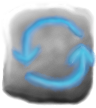
\includegraphics[width=0.4\textwidth]{images/switch_on.png}
        
\includegraphics[width=0.4\textwidth]{images/switch_on_50.png}
        \caption{Przykład obrazu rastrowego po skalowaniu: \\ Po lewej stronie - oryginalny obraz, \\ Po prawej stronie - obraz zmniejszony czterokrotnie}
        \label{RasterGraphics_1}
\end{figure}

\newpage
\par Poza kwestią skalowania, możliwość edycji nawet pojedynczych pikseli niesie za sobą wiele zalet. Dzięki takiemu rozwiązaniu można narysować praktycznie wszystko, ponieważ w~programach do edycji grafiki rastrowej takich jak na przykład \textit{Photoshop} czy \textit{Gimp 2}, istnieją dziesiątki narzędzi, które dają praktycznie nieograniczone możliwości. Jednym z~najprostrszych narzędzi jest pędzel - podstawy przyrząd - za którego pomocą powstaje większość grafiki. Wysoką jakość obrazu można osiągnąć używając tzw. miękkich krawędzi pędzla (zob. rysunek \ref{RasterGraphics_2}). Jeśli pędzel rysuje obiekty w~kształcie koła, miękkimi krawędziami będą zewnętrzne okręgi koła o~odpowiednim stopniu przeźroczystości. Częściowa przeźroczystość pozwala na "wtapianie" w~siebie różnych elementów obrazu, maskując przy tym ostre krawędzie tworzone przez piksele. Kolejną techniką pozwalającą na osiągnięcie podobnego efektu jest używanie wszelakich narzędzi wygładzających, które powodują stopniowe wyrównywanie wartości barw. Takie wyrównywanie powoduje większe ujednolicenie kolorów, co owocuje gładszym przejściem pomiędzy pikselami.

\begin{figure}[hpt!]
        \centering
        
\includegraphics[width=0.8\textwidth]{images/smooth.png}
        \caption{Przykład zastosowania miękkich krawędzi pędzla - po prawej stronie, \\ oraz twardych krawędzi - po lewej stronie}
        \label{RasterGraphics_2}
\end{figure}

\paragraph{Grafika wektorowa}\hfill \break

\par W~przeciwieństwie do grafiki rastrowej, wektorowa nie jest tworzona za pomocą pikseli. Obiekty kreowane za pomocą grafiki wektorowej opisywane są za pomocą równań geometrycznych. Dzięki takiej budowie grafiki wektorowe są odporne na utratę jakości podczas skalowania (zob. rysunek \ref{VectorGraphics}), ponieważ sama budowa obiektów się nie zmienia, a~jedynie ich wyjściowe wymiary. Z~pewnego punktu widzenia grafika rastrowa przypomina malowanie czegoś nowego, natomiast grafika wektorowa budowanie z~istniejących już elementów. Dzięki takiej konstrukcji obrazy wektorowe znajdują szczególne zastosowanie na przykład w~dziedzinie web development'u, gdzie logo firmy umieszczone na stronie zawsze jest w~dobrej jakości, a~przy odpowiednim dostosowaniu \textit{responsywności}\footnote{Dostosowanie obrazu do wielkości wyświetlacza na którym jest prezentowana}, również zawsze w~adekwatnym rozmiarze.

\begin{figure}[hpt!]
        \centering
        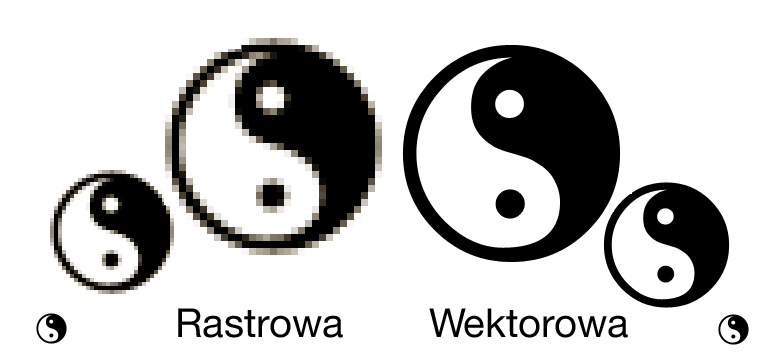
\includegraphics[width=0.8\textwidth]{images/rastrowa-wektorowa.jpg}
        \caption{Różnica w~skalowaniu grafik wektorowej i~rastrowej. Źródło: \cite{Vector}}
        \label{VectorGraphics}
\end{figure}


\subsection{Grafika 3D}

\par Grafika 3D łączy w~sobie aspekty zarówno grafiki rastrowej jak i~wektorowej. Przestrzeń w~jakiej są tworzone obiekty jest przestrzenią trójwymiarową (zob. rysunek \ref{3DGraphics_2}), zamiast dwuwymiarowego "płótna", ale zasada działania jest podobna do tej wykorzystywanej w~grafice wektorowej. Obiekty również są opisywane równaniami matematycznymi, a~ich składowe takie jak wierzchołki, ściany czy krawędzie posiadają swoje parametry. Dzięki tym parametrom można określić wymiary oraz położenie w~przestrzeni zarówno całych obiektów jak i~ich składowych. Pomimo przestrzeni posiadającej trzy wymiary jesteśmy w~stanie tworzyć obiekty dwuwymiarowe, służące na przykład jako tło scenerii. Najczęściej jednak grafika rastrowa w~trójwymiarze znajduje zastosowanie w~postaci tekstur dla obiektów 3D. W~przypadku grafiki 3D bardzo ważnym aspektem jest również oświetlenie - coś nieobecnego w~grafice 2D. Odpowiednio ustawione oświetlenie daje niesamowite możliwości oraz znacznie poprawia jakość finalnego produktu, dzięki bardziej realistycznemu wyglądowi.

\begin{figure}[hpt!]
        \centering
        \quad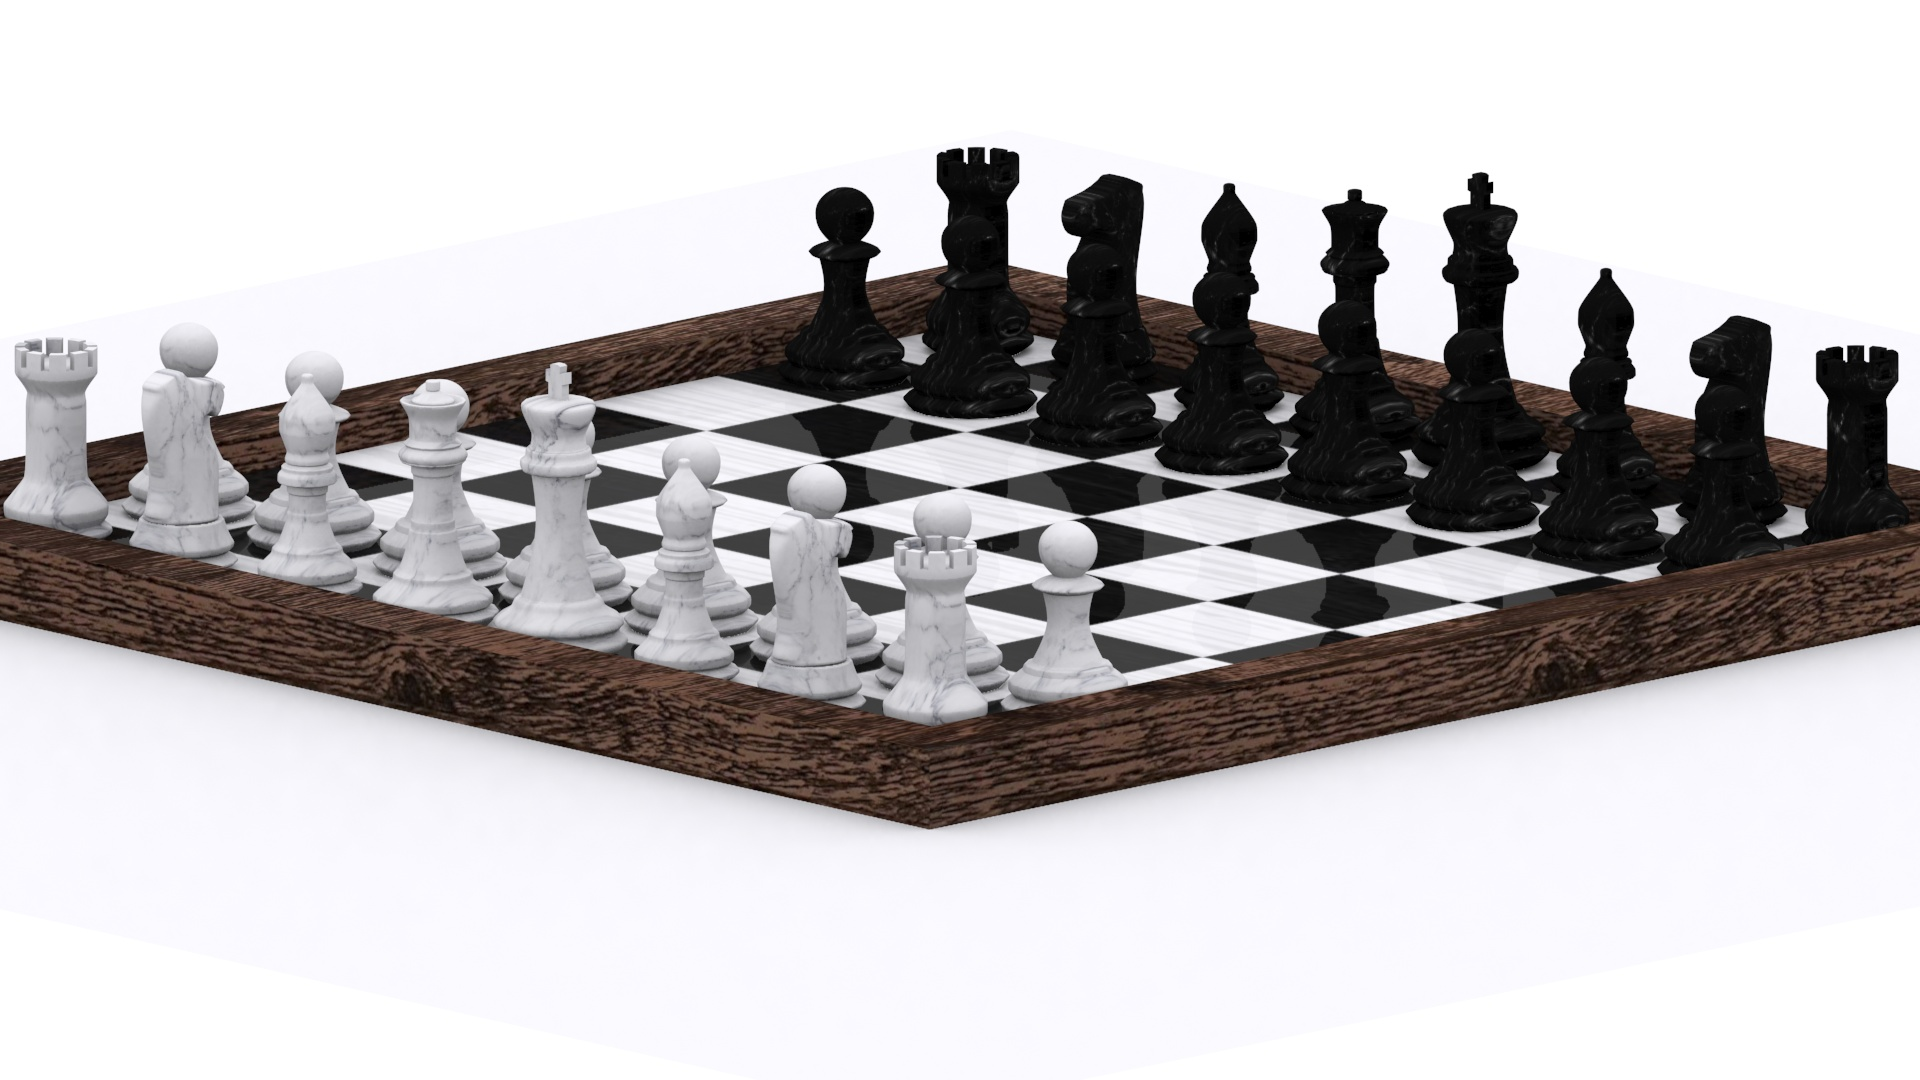
\includegraphics[width=0.6\textwidth]{images/Chess_1.jpg}A)
        \quad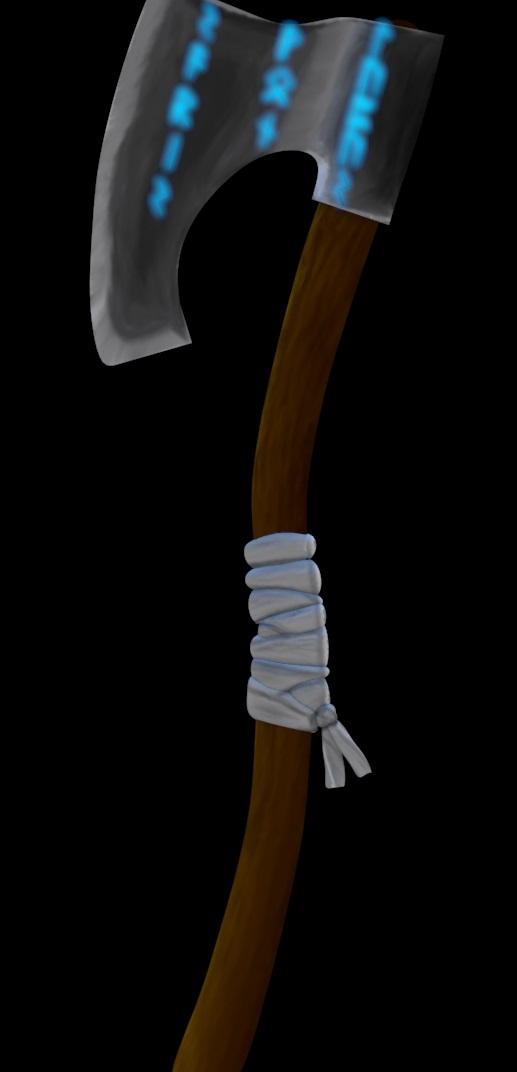
\includegraphics[width=0.2\textwidth]{images/3D_Axe.jpg}B)
        \caption{Przykłady obiektów trójwymiarowych}
        \label{3DGraphics_2}
\end{figure}

\section{Grafika w~grach komputerowych}

\subsection{Graficzne aspekty gier}

\par W~grach komputerowych grafika jest praktycznie wszechobecna, wykorzystuje się ją w~zasadzie na każdym etapie produkcji, czy promocji gry. Zależnie od rodzaju gry, może być wykorzystywana grafika 2D lub 3D, najczęściej jednak obie. Więcej zastosowań znajduje grafika 2D, jednak to nie umniejsza znaczeniu obiektów 3D, które bardzo często zajmują więcej czasu podczas tworzenia, przez swoją wysoką złożoność. Obrazy dwuwymiarowe występują w~grach między innymi jako:

\begin{itemize}

\item \textit{Tekstury} (zob. rysunek \ref{Textures}) - w~przypadku gier 2D są to obrazy tworzące elementy otoczenia, postacie oraz przedmioty. W~grafice 3D tekstury są obrazami specjalnie rozłożonymi na płaszczyźnie tak, aby po nałożeniu ich na obiekt 3D poprawnie go pokrywały.

\begin{figure}[hpt!]
        \centering
        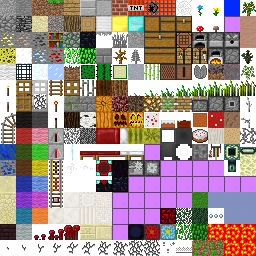
\includegraphics[width=0.8\textwidth]{images/tex2D.png}
        \caption{Przykładowe tekstury i~przedmioty. Źródło: \cite{Textures}}
        \label{Textures}
\end{figure}

\item \textit{Tła} (zob. rysunek \ref{Background}) - są to obrazy mające na celu nadanie głębi grom, takim jak gry platformowe; zależnie od wielu czynników mogą być bardzo złożone jak i~bardzo proste, ponieważ nie są czymś co gracz widzi na pierwszym planie, są pewnego rodzaju wypełnieniem, akcentem.

\begin{figure}[hpt!]
        \centering
        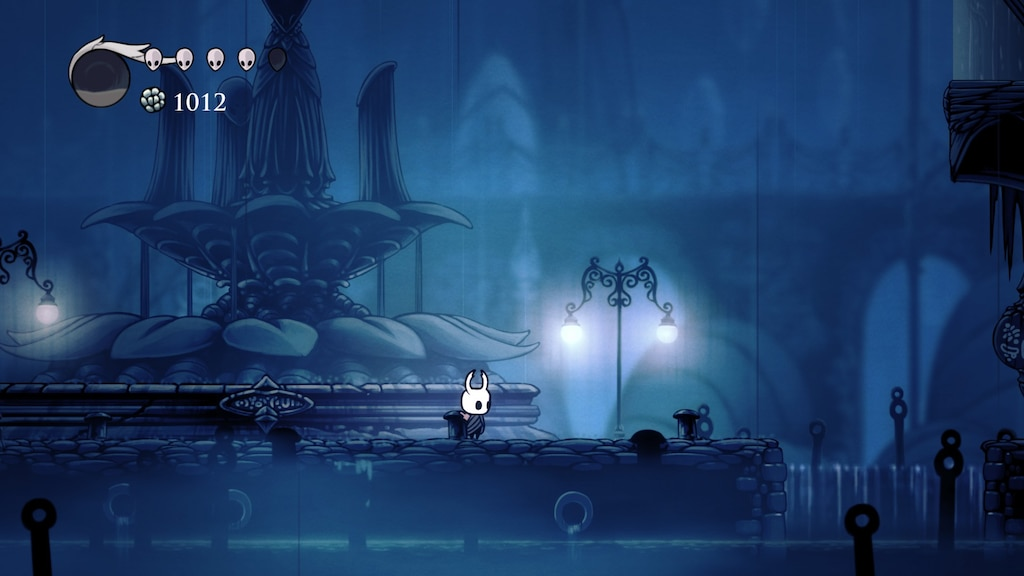
\includegraphics[width=0.8\textwidth]{images/bckGr.jpg}
        \caption{Przykład tła w~grze. Źródło: \cite{Background}}
        \label{Background}
\end{figure}

\item \textit{Ekrany ładowania} (zob. rysunek \ref{LoadingScreen}) - niezależnie od rodzaju gry, ekrany ładowania mają na celu umilenie czasu, jaki gracz musi odczekać przed załadowaniem się poziomu. Często przedstawiają ciekawe widoki ze świata gry, potwory z~jakimi przyjdzie graczowi się zmierzyć, albo różne ciekawostki, czy wskazówki dotyczące rozgrywki. W~niektórych grach za pomocą ekranów ładowania prowadzona jest narracja - tekst, często w~towarzystwie czytającego go lektora, lub filmy czy animacje.

\begin{figure}[hpt!]
        \centering
        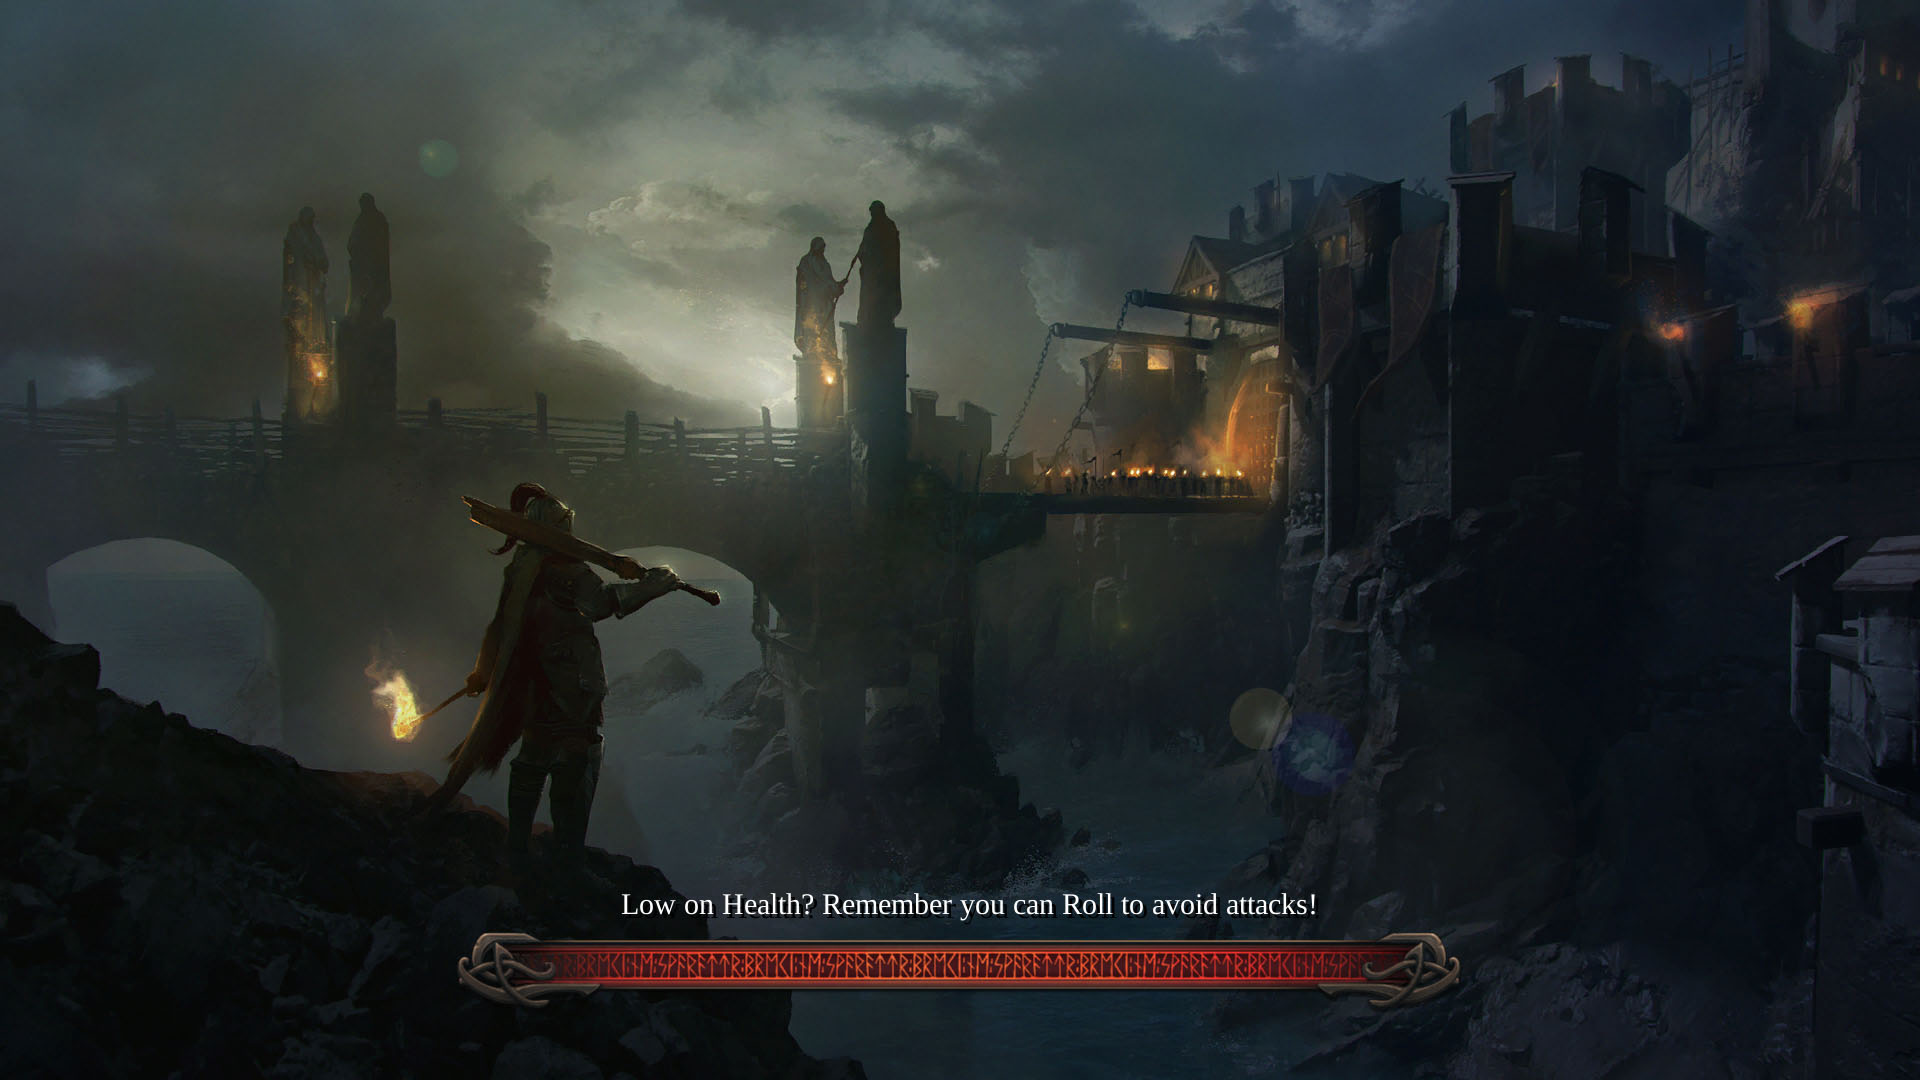
\includegraphics[width=0.8\textwidth]{images/loadSCR.jpg}
        \caption{Przykład ekranu ładowania. Źródło: \cite{loadSCR}}
        \label{LoadingScreen}
\end{figure}

\item \textit{Elementy interfejsu} (zob. rysunek \ref{Interface}) - do tej kategorii elementów graficznych należą różnego rodzaju przyciski, obramowania okien, kursory, a~nawet specjalnie robione na potrzeby gry czcionki.

\begin{figure}[hpt!]
        \centering
        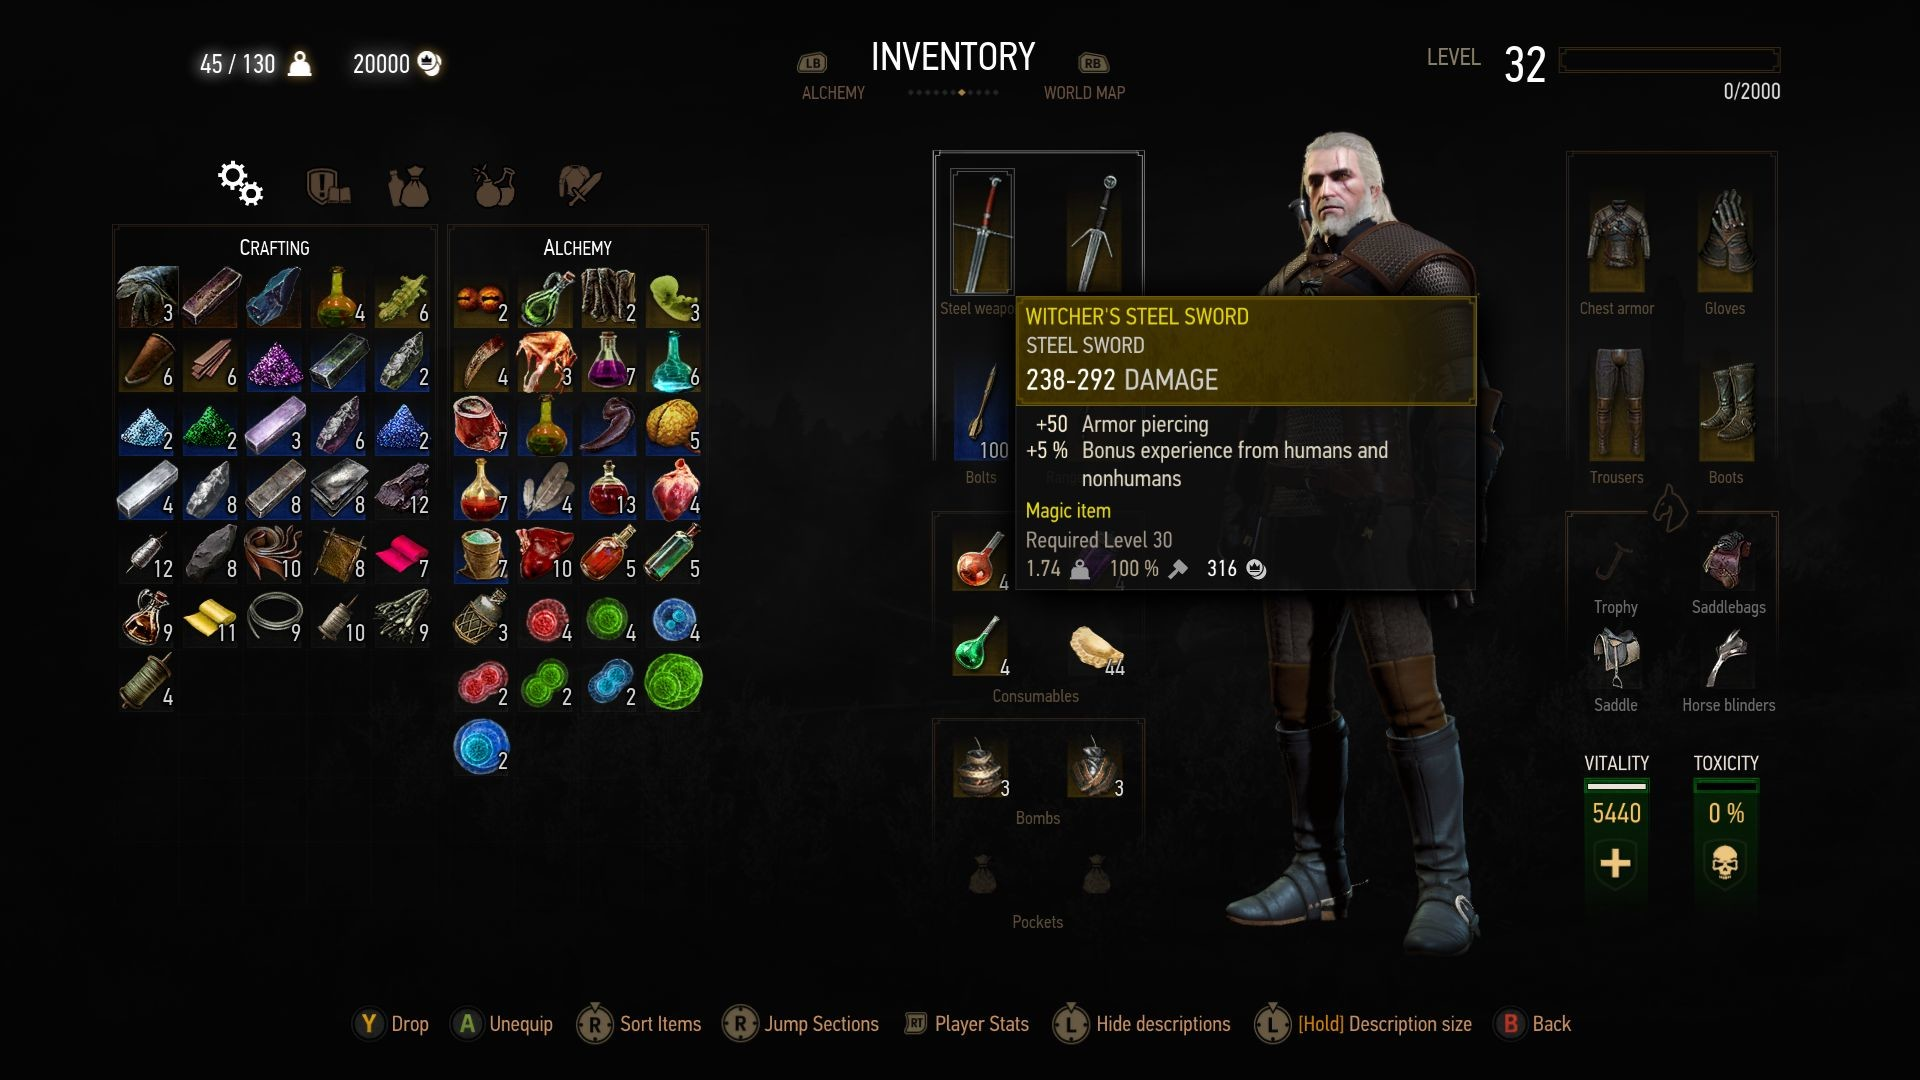
\includegraphics[width=0.8\textwidth]{images/interface.jpg}
        \caption{Przykładowy interfejs. Źródło: \cite{interface}}
        \label{Interface}
\end{figure}

\end{itemize}

\par Poza szerokim zakresem zastosowań grafik 2D podczas produkcji gier, istnieje również inny obszar, który tak naprawdę opiera się na grafikach i~animacjach związanych z~grą - promocja gry. Do promocji gry najczęściej wykorzystywane spośród grafik są tak zwane \textit{Concept Arty} (zob. rysunek \ref{ConceptArt}), czyli grafiki koncepcyjne przedstawiające to, jak gra ma docelowo wyglądać lub co ma oferować. Warto również wspomnieć, że wszystkie grafiki używane podczas produkcji, czy promocji gier są grafikami rastrowymi, wyjątki stanowią jedynie obrazy, takie jak logo gry zamieszczone na stronie dotyczącej produktu.

\begin{figure}[hpt!]
        \centering
        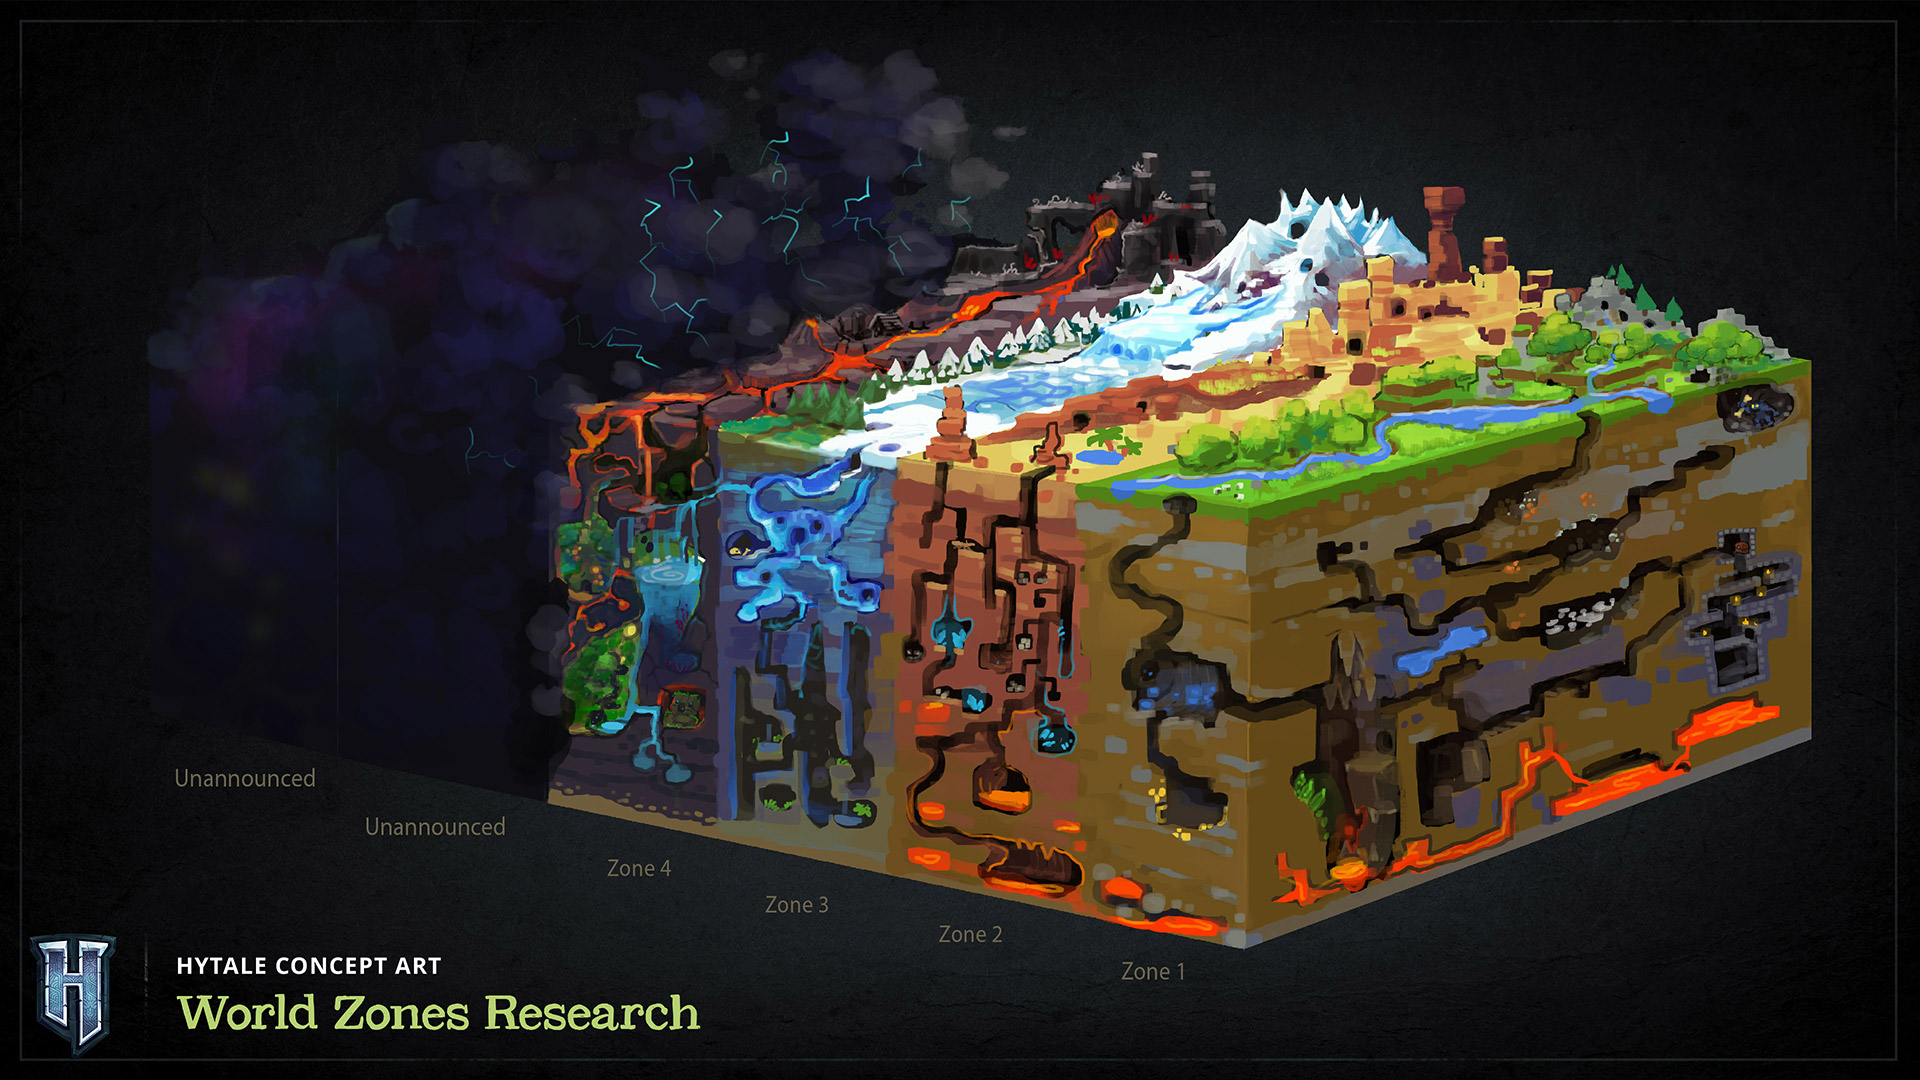
\includegraphics[width=0.8\textwidth]{images/conceptArt.jpg}
        \caption{Przykład grafiki koncepcyjnej. Źródło: \cite{conceptArt}}
        \label{ConceptArt}
\end{figure}

\subsection{Animacje}

\par Animacje są bardzo ważnym aspektem w~produkcji gier komputerowych. Tak jak zwykłe grafiki, mogą być bardzo zaawansowane, jak i~bardzo proste. Najprostszymi animacjami są \textit{animacje poklatkowe}, które są po prostu zbiorem grafik przedstawiających kilka stadiów ruchu. Takie grafiki są wyświetlane po sobie bardzo szybko, co powoduje złudzenie optyczne wyglądające jak ruch. Do uzyskania takiego efektu można wykorzystać zaledwie trzy grafiki, ale można użyć ich o~wiele więcej, co znacząco zwiększy płynność animacji. Innym rodzajem animacji wykorzystywanym w~grach są animacje tworzone przy użyciu programów do grafiki 3D takich jak \textit{3Ds max}, czy \textit{Blender}. Na potrzeby animacji tworzy się całe sceny, a~następnie przy pomocy odpowiednich narzędzi wyznacza się tak zwane \textit{klatki kluczowe}, w~których zmienia się na przykład położenie, czy kształt obiektów. Po wyznaczeniu klatek kluczowych program sam wylicza parametry obiektów dla klatek pośrednich, tak żeby przejście pomiędzy jedną klatką kluczową, a~drugą było płynne. Takie rozwiązanie wydaje się być prostsze i~mniej czasochłonne od klasycznych animacji poklatkowych, ale za to wymaga o~wiele większej mocy obliczeniowej.

\section{Grafika w~grze "Tree of Life"}

\par "Tree of Life" jest dwuwymiarową grą platformową, dlatego do jej stworzenia została wykorzystana jedynie grafika 2D, a~konkretnie rastrowa. Wszystkie obrazy zostały wykonane w~programie \textit{Gimp 2} oraz wyeksportowane w~formacie \textit{PNG}.
\par Gry platformowe często posiadają poziomy o~różnej tematyce, co oznacza, że lokacje różnią się motywem przewodnim jak np. las, jaskinie, czy zima. Pomimo tych różnic między lokacjami, budowane one są w~ten sam sposób - z~modułowych platform (zob. rysunek \ref{PlatformTexture}). Wspomniane platformy tworzy się za pomocą pojedynczych bloków, które pokrywa ta sama tekstura. W~"Tree of Life" platformy zbudowane są przy użyciu 4 wariantów tej samej tekstury - lewa i~prawa krawędź, środek oraz pojedynczy, samodzielny blok. Model postaci (zob. rysunek \ref{HeroSkin}) został utworzony na podobnej zasadzie co platformy - zbiór kilku grafik, używanych zależnie od stanu postaci, w~jaki wprawia ją gracz. Ruchy postaci osiągane są przy użyciu najprostszej animacji poklatkowej - szybka zmiana obrazów przedstawiająca różne pozy bohatera. 


\begin{figure}[hpt!]
        \centering
        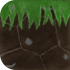
\includegraphics[width=0.3\textwidth]{images/grass_L.png}
        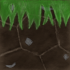
\includegraphics[width=0.3\textwidth]{images/grass_C.png}
        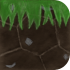
\includegraphics[width=0.3\textwidth]{images/grass_R.png}
        \caption{Przykład modułów platformowych.}
        \label{PlatformTexture}
\end{figure}

\begin{figure}[hpt!]
        \centering
        
\includegraphics[width=0.2\textwidth]{images/player_standR.png}
        
\includegraphics[width=0.2\textwidth]{images/player_walkR1.png}
        
\includegraphics[width=0.2\textwidth]{images/player_walkR2.png}
        
\includegraphics[width=0.2\textwidth]{images/player_jumpR.png}
        \caption{Przykład różnych pozycji bohatera.}
        \label{HeroSkin}
\end{figure}
\newpage
\paragraph{Model RGB}\hfill \break
\par W~modelu barw \textit{RGB - Red Green Blue} (zob. rysunek \ref{RGB}) kolory powstają poprzez połączenie świateł o~kolorach czerwonym, zielonym oraz niebieskim. Każdemu z~kolorów początkowych można przypisać wartość od 0 do 255, a~ponieważ model \textit{RGB} jest modelem \textit{addytywnym}, przypisanie każdej składowej wartości równej 0 da kolor czarny - brak światła, natomiast po przypisaniu wartości 255 dla każdej składowej, otrzymamy kolor biały - pełne światło. Dzięki tak dużemu zakresowi przypadającemu na każdy z~kolorów bazowych można uzyskać ponad 16 milionów barw, co daje ogromne możliwości podczas tworzenia obrazów.

\begin{figure}[hpt!]
        \centering
        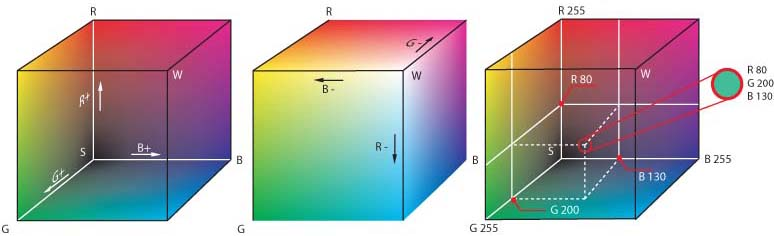
\includegraphics[width=0.8\textwidth]{images/RGB.jpg}
        \caption{Graficzna prezentacja modelu RGB. Źródło: \cite{RGB}}
        \label{RGB}
\end{figure}

\paragraph{Format PNG}\hfill \break
\par Format \textit{PNG} charakteryzuje bezstratna kompresja danych, która pozwala na wykorzystanie pełnej gamy kolorów modelu \textit{RGB} bez straty na jej jakości. W~\textit{PNG} dostępny jest również \textit{Kanał Alfa}, który umożliwia zastosowanie przeźroczystości. Dzięki jej wykorzystaniu postać w~grze nie przypomina prostokąta, pomimo iż "płótno", na którym zastała narysowana jest w~kształcie prostokąta. Takie rozwiązanie pozwala również na gładkie wtapianie w~siebie różnych grafik, a~tym samym mniejszą widoczność pojedynczych pikseli.  

\paragraph{Gimp 2}\hfill \break
\par \textit{Gimp 2} to zaawansowany program do edycji grafiki rastrowej, posiadający dziesiątki narzędzi dających niemal nieograniczone możliwości. Do tworzenia grafik użytych w~grze "Tree of Life" zostały wykorzystane między innymi następujące przybory:

\begin{itemize}

\item \textit{Pędzel} - Najbardziej podstawowe narzędzie w~programach do grafiki rastrowej.

\item \textit{Rozsmarowywanie} - Narzędzie służące do rozmywania pikseli ze sobą sąsiadujących, w~odpowiednim kierunku.

\item \textit{Rozjaśnianie/Przyciemnianie} - Za pomocą tego przyboru można rozjaśniać lub przyciemniać punktowo obszary obrazu, dzięki czemu można uzyskać na przykład efekt cienia.

\par Poza  powyższymi narzędziami, w~dużym stopniu została wykorzystana budowa warstwowa obrazu, dzięki której można pracować na jednym elemencie obrazu, nie ingerując w~pozostałe.

\end{itemize}

%############################################################################################
%############################################################################################
%-----------   Rozdział 4. Techniczne aspekty tworzenia gier komputerowych       -----------# 
%############################################################################################
%############################################################################################

\chapter{Techniczne aspekty tworzenia gier komputerowych}
\par Rozdział ten porusza kwestie związane z częścią programistyczną gier komputerowych. Opisane zostaną silniki oraz biblioteki służące do ich tworzenia oraz przedstawione w tej produkcji algorytmy. Przedstawiona zostanie również struktura projektu oraz sposoby testowania gry.

\section{Silniki gier komputerowych}
\par Obecnie na rynku istnieje wiele firm specjalizujących się w~tworzeniu gier komputerowych. Wykorzystują one najróżniejsze technologie, aby ich produkcje były chętnie nabywane przez użytkowników. Jednym z~ważniejszych elementów powstania dobrej produkcji jest dobranie odpowiedniego \textit{silnika gry}, czyli głównej części kodu gry komputerowej, który jest dostępny razem z~odpowiednim środowiskiem programistycznym. Jego głównym zadaniem jest ułatwienie pracy podczas tworzenia poszczególnych elementów oraz interakcję między nimi. Czasami zdarza się, że silnik gry ma wbudowane w~siebie moduły do obsługi grafik, sieci oraz sztucznej inteligencji.
\par Istnieje bardzo duża ilość dostępnych silników umożliwiających programistom tworzenie gier komputerowych. Można tutaj wyróżnić:
\begin{itemize}
    \item \textit{Unity} - jest to jeden z~najpopularniejszych silników. Stworzony przez firmę \textit{Unity Technologies} i~opublikowany w~2005 roku. Jego zaletą jest obsługiwanie większości platform dostępnych na rynku. Jest on doskonały dla początkujących twórców, ponieważ jest bardzo intuicyjny. Dla twórców, których dochody nie przekraczają 100 tysięcy dolarów rocznie jest on darmowy.
    \item \textit{Source Engine} - jest to silnik objęty prawami zamkniętego oprogramowania, stworzony przez firmę \textit{Valve}. Swoją premierę miał w~2004 roku wraz z~wydaniem kultowej gry \textit{Half-Life 2}. Z~biegiem lat był on ulepszany o~coraz to nowe funkcjonalności, w~efecie czego w~oparciu o~niego powstało wiele popularnych tytułów: \textit{Counter-Strike: Global Offensive}, \textit{Dota 2} oraz wiele innych.
    \item \textit{Unreal Engine} - wydany w~1998 roku przez firmę \textit{Epic Games} wraz z~grą \textit{Unreal} silnik \textit{Unreal Engine} jest jednym z~najpopularniejszych silników gier na świecie. Wprowadzono w~nim \textit{schematy}, które umożliwiają pracę z~nim nawet osobom nieznającym języka programowania \textit{C++}.
    \item \textit{REDengine} - jest to silnik opracowany przez polskie studio \textit{CD Projekt RED} na potrzeby ich własnych produkcji. Wykorzystany został w~grach z~serii \textit{Wiedźmin} oraz w~grze \textit{Cyberpunk 2077}. Jego główną zaletą jest możliwość projektowania złożonej oraz nieliniowej fabuły.
\end{itemize}

\section{Biblioteki do tworzenia gier komputerowych}
\par Obok silników gier komputerowych na rynku dostępne są również biblioteki służące do ich tworzenia. Mimo ich małej popularności oraz większego skomplikowania podczas procesu powstawiania gry, na ich podstawie również powstało kilka produkcji, które zawładnęły rynkiem gier. 
\subsection{The Lightweight Java Game Library}
\par Czołowym tytułem, który powstał dzięki bibliotece służącej do produkcji gier jest najpopularniejsza produkcja na świecie \textit{Minecraft Java Edition}(zob. rys. 4.1). Tytuł ten został napisany w~oparciu o~bibliotekę \textit{The Lightweight Java Game Library}, w~skrócie \textit{LWJGL}. Jest to biblioteka dla języka \textit{Java}, która zawiera w~sobie biblioteki powszechnie stosowane podczas tworzenia gier takie jak: \textit{OpenGL}, \textit{Vulkan}, \textit{OpenAL} oraz \textit{OpenCL}. Zapewnia również dostęp do urządzeń peryferyjnych umożliwiających sterowanie grą.
\begin{figure}[hpt!]
        \centering
        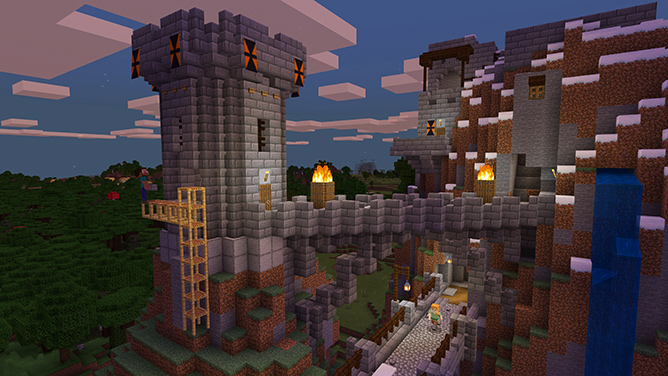
\includegraphics[width=0.8\textwidth]{images/minecraft.jpg}
        \caption{Przykładowy zrzut ekranu z~gry Minecraft Java Edition. Źródło: \cite{Minecraft}}
        \label{Minecraft}
\end{figure}
\newpage
\subsection{Biblioteka Pygame}
\par W~projekcie \textit{TreeOfLife} wykorzystana została biblioteka \textit{pygame}. Stworzona została przez \textit{Pete Shinnersa} w~oparciu o~biblioteki \textit{SDL}. Jest ona udostępniona na zasadach wolnego oprogramowania i~dystrybuowana na licencji \textit{LGPL}\footnote{\textit{LGPL} - licencja bardzo podobna do GPL, jednak w~przeciwieństwie do niej nakłada ograniczenia tylko na poszczególne pliki źródłowe, a~nie na cały program}. Została ona napisana w~języku programowania \textit{Python}, który obecnie jest jednym z~popularniejszych na rynku. Pozwala ona na wyświetlanie na ekranie grafik 2D oraz obsługę klawiatury czy też myszy. Jest ona bardzo prosta w~obsłudze, co jest jej dużą zaletą. W~przeciwieństwie do innych tego typu bibliotek, nie ma aż tak dużej liczby wbudowanych funkcji, więc aby osiągnąć zamierzony efekt programista musi zdać się na swoje umiejętności i~wyobraźnię.

\section{Algorytmy i~struktury użyte w~grze "Tree Of Life"}
\par Podczas procesu tworzenia gry \textit{Tree Of Life} wykorzystany został system kontroli wersji - git. Dzięki zastosowaniu tego narzędzia możliwe było wersjonowanie powstałego kodu. Pełny kod programu oraz przedstawione algorytmy znajdują się w~repozytorium Github\cite{Github}. Mimo niewielkiej ilości poziomów w~grze wykorzystanych zostało około 160 grafik. Za działanie całego programu odpowiada 32 klasy oraz około 3000 linii kodu.

\subsection{Przeliczanie Binarne}
\par \textit{Przeliczanie Binarne} jest podstawową operacją używaną w~informatyce. W~systemie dwójkowym liczby zapisujemy za pomocą cyfr 0 i~1. \textit{System dwójkowy} jest używany w~implementacji sprzętowej, która odpowiada stanom "włączony" i~"wyłączony", jak również w~celu zminimalizowania przekłamania danych. 

\subsection{Sortowanie bąbelkowe}
\par \textit{Sortowanie bąbelkowe} jest jednym z~najstarszych algorytmów służących do sortowania. Jest to nieefektywny algorytm, ponieważ jego czasowa złożoność obliczeniowa jest rzędu $O(n^2)$, gdzie \textit{n} oznacza rozmiar sortowanej tablicy. Polega on na zamianie sąsiadujących ze sobą elementów do czasu napotkania większego od niego elementu. W~pesymistycznym przypadku program ten z~każdym kolejnym krokiem będzie miał o~jeden element mniej do porównania. Sytuacja ta będzie miała miejsce, gdy danymi wejściowymi będzie otrzymana tablica posortowana w~sposób odwrotny do oczekiwanego.

\subsection{Szyfr PlayFair}
\par \textit{Szyfr PlayFair} jest jednym z~prostszych algorytmów szyfrujących. Został on wynaleziony w~1854 roku przez \textit{sir Charlesa Wheatstone'a}, spopularyzował go \textit{baron Lyon Playfair}, skąd wzięła się jego nazwa. Był on używany podczas \textit{I wojny światowej} przez armię brytyjską. Polega on na podziale tekstu wejściowego na pary liter - gdy długość tekstu jest nieparzysta, na koniec ciągu znaków należy dodać literę na przykład 'z' - oraz zamianie ich na inną parę liter według ściśle określonych zasad:
\begin{itemize}
    \item Jeżeli obie litery znajdują się w~tym samym wierszu, zamieniane zostają na litery sąsiadujące z~prawej strony według tablicy szyfrującej - jeżeli litera będzie znajdować się w~ostatniej kolumnie należy zastąpić ją znakiem z~pierwszej kolumny,
    \item Jeżeli obie litery znajdują się w~tej samej kolumnie, zamieniane zostają na litery sąsiadujące z~dołu według tablicy szyfrującej - jeżeli litera będzie znajdować się w~ostatnim wierszu, należy zastąpić ją znakiem z~pierwszego wiersza,
    \item w~pozostałych przypadkach daną parę liter należy zastąpić znakami leżącymi na przecięciu wierszy i~kolumn, w~jakich dane wejściowe się znajdują.
\end{itemize}
\par Do szyfrowania użyta zostaje również tablica szyfrująca, która składa się z~niepowtarzających się liter alfabetu. Może zostać zastosowany również klucz szyfrowania - słowo, które umieszcza się na początku danej tablicy szyfrowania, a~resztę znaków ustawia się zgodnie z~zasadą niepowtarzalności w~kolejności alfabetycznej na dalszych miejscach tablicy (zob. rysunek \ref{TablicaSzyfrowania}). 
\par Proces odszyfrowania danego szyfrogramu polega na odwróceniu działań związanych z~szyfrowaniem, czyli: litery, które zamieniane były na te sąsiadujące z~prawej-zamieniane są na te z~lewej, te zamieniane na te z~dołu, na te z~góry.
\begin{figure}[hpt!]
        \centering
        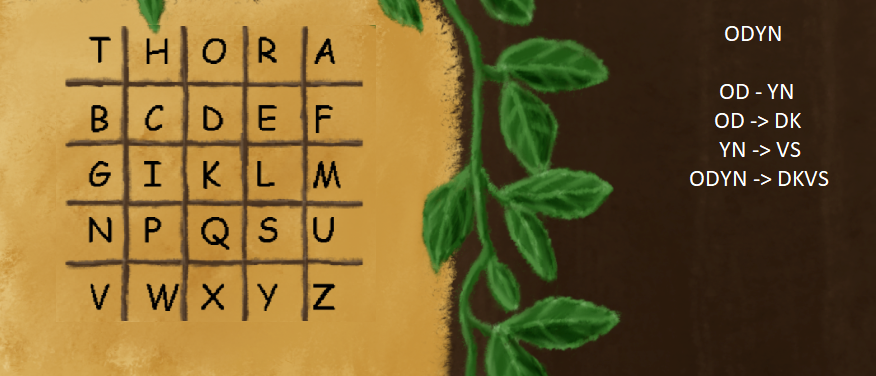
\includegraphics[width=0.8\textwidth]{images/PLAYFAIR_PRZYKLAD.png}
        \caption{Przykładowy proces szyfrowania za pomocą szyfry PlayFair z kluczem}
        \label{TablicaSzyfrowania}
\end{figure}

\subsection{Drzewa Binarne}
\par \textit{Drzewa Binarne} (zob. rysunek \ref{BinaryTree}) są dynamicznymi strukturami danych tworzonymi zgodnie z~zasadą, że każde lewe poddrzewo zawiera elementy mniejsze od \textit{węzła}\footnote{\textit{węzeł} - element nadrzędny dla poddrzew}, natomiast prawe poddrzewo zawiera elementy większe od tegoż elementu. Każdy z~węzłów oprócz wartości (klucza), przechowuje również wskaźniki na swojego lewego i~prawego potomka jak również i~na swojego przodka\footnote{\textit{przodek} - element nadrzędny dla danego węzła}. Każde drzewo binarne posiada tzw. \textit{korzeń} - pierwszy węzeł, który nie posiada elementu nadrzędnego. W~przeciwieństwie do innych typów drzew, drzewo binarne może posiadać co najwyżej dwoje dzieci - poddrzew. 
\begin{figure}[hpt!]
        \centering
        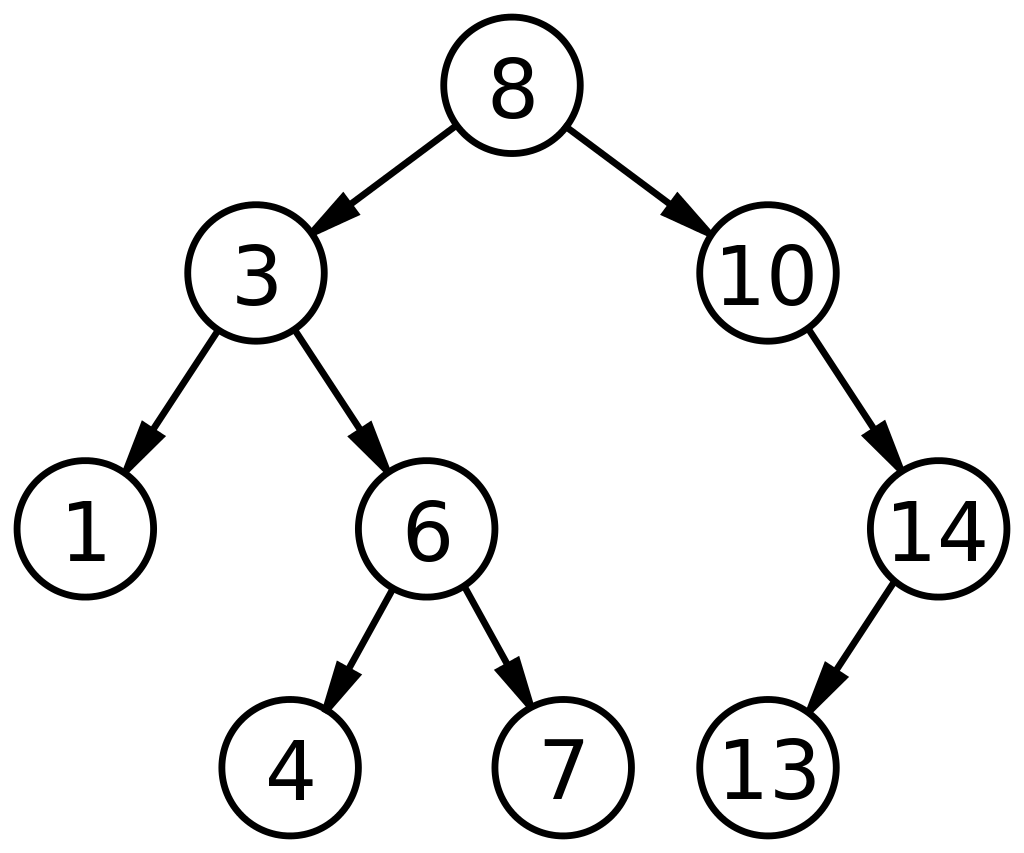
\includegraphics[width=0.8\textwidth]{images/Binary_search_tree.svg.png}
        \caption{Przykładowe drzewo binarne o~wysokości 3. Źródło: \cite{BinaryTree}}
        \label{BinaryTree}
\end{figure}
\section{Struktura projektu}
\par W~projekcie \textit{Tree Of Life} (zob. rysunek \ref{StrukturaAll}) można wyodrębnić następujące funkcjonalne części:

\begin{figure}[hpt!]
        \centering
        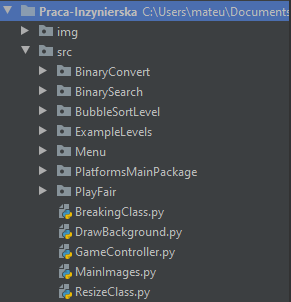
\includegraphics[width=0.5\textwidth]{ProjectStructure/strukturaAll.png}
        \caption{Struktura katalogów Projektu}
        \label{StrukturaAll}
\end{figure}
\newpage
\begin{itemize}
    \item Moduł \textit{BinaryConvert} (zob. rysunek \ref{StrukturaBinConv}) zawierający operacje związane z~poziomem przeliczania binarnego. Wyróżnia się tu:
        \begin{itemize}
            \item \textit{ActionClass.py} - klasa zawierająca zdefiniowane akcje dozwolone dla gracza,
            \item \textit{BinaryConvertMain.py} - główna klasa poziomu,
            \item \textit{Numbers.py} - klasa, w~której zdefiniowane są operacje sprawdzające poprawność rozwiązania,
            \item \textit{Pins.py} - klasa reprezentująca wyświetlane "piny" na ekranie,
        \end{itemize}
        \begin{figure}[hpt!]
            \centering
            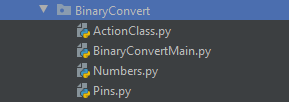
\includegraphics[width=0.5\textwidth]{ProjectStructure/strukturabinconv.png}
            \caption{Struktura Modułu BinaryConvert}
            \label{StrukturaBinConv}
        \end{figure}
    
    \item Moduł \textit{BinarySearch} (zob. rysunek \ref{StrukturaBinarySearch}) zawierający operacje związane z~ostatnim poziomem w~grze. Wyróżnia się tu:
        \begin{itemize}
            \item \textit{BinaryPlatforms.py} - zawiera klasę reprezentującą platformy,
            \item \textit{BinarySearchMain.py} - główna klasa poziomu,
            \item \textit{GenerateTree.py} - klasa odpowiedzialna za tworzenie drzewa binarnego,
            \item \textit{ShowAnswer.py} - klasa mająca na celu wyświetlanie przebytej drogi przez użytkownika,
        \end{itemize}
        \begin{figure}[hpt!]
            \centering
            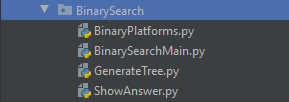
\includegraphics[width=0.5\textwidth]{ProjectStructure/strukturaBinarySearch.png}
            \caption{Struktura Modułu BinarySearch}
            \label{StrukturaBinarySearch}
        \end{figure}
    \item Moduł \textit{BubbleSortLevel} (zob. rysunek \ref{StrukturaBubbleSort}) zawierający operacje związane z~poziomem sortowania bąbelkowego. Wyróżnia się tu:
        \begin{itemize}
            \item \textit{BubbleSortLevelMain.py} - główna klasa poziomu,
            \item \textit{SwitchingButtons.py} - klasa odpowiedzialna za wyświetlane na ekranie przyciski,
            \item \textit{SwitchingNumbers.py} - klasa zawierająca operacje związane z~cyframi wyświetlanymi na ekranie,
        \end{itemize}
        \begin{figure}[hpt!]
            \centering
            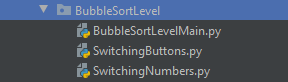
\includegraphics[width=0.5\textwidth]{ProjectStructure/strukturabubble.png}
            \caption{Struktura Modułu BubbleSortLevel}
            \label{StrukturaBubbleSort}
        \end{figure}
    
    \item Moduł \textit{ExampleLevels} (zob. rysunek \ref{StrukturaExampleLevels}) zawierający definicje poszczególnych poziomów platformowych. Wyróżnia się tu:
        \begin{itemize}
            \item \textit{ExampleLvl.py} - definicja poziomu w~lokacji \textit{SVARTAL},
            \item \textit{ExampleLvl2.py} - definicja poziomu w~lokacji \textit{ANCIENT FOREST},
        \end{itemize}
        \begin{figure}[hpt!]
            \centering
            
\includegraphics[width=0.5\textwidth]{ProjectStructure/strukturaExampleLvl.png}
            \caption{Struktura Modułu ExampleLevels}
            \label{StrukturaExampleLevels}
        \end{figure}
    
        \item Moduł \textit{Menu} (zob. rysunek \ref{StrukturaMenu}) zawierający klasę odpowiedzialną za ekrany rozpoczęcia i~zakończenia rozgrywki. Wyróżnia się tu:
        \begin{itemize}
            \item \textit{Menu.py} - klasa służąca do obsługi rozpoczęcia i~zakończenia rozgrywki,
        \end{itemize}
        \begin{figure}[hpt!]
            \centering
            
\includegraphics[width=0.5\textwidth]{ProjectStructure/strukturaMenu.png}
            \caption{Struktura Modułu Menu}
            \label{StrukturaMenu}
        \end{figure}
    
            \item Moduł \textit{PlatformsMainPackage} (zob. rysunek \ref{StrukturaPlatforms}) zawierający pliki odpowiedzialne za poszczególne elementy w~poziomach platformowych. Wyróżnia się tu:
        \begin{itemize}
            \item \textit{BaseLevelPlatform.py} - główna klasa poziomów platformowych,
            \item \textit{BulletClass.py} - klasa odpowiadająca za pociski tworzone przez gracza bądź przeciwników,
            \item \textit{CeilingClass.py} - klasa, która użyta będzie podczas rozwijania gry - odpowiada za sufit - zachowanie gracza, aby postać nie znikała poza ekranem gry,
            \item \textit{EnemyClass.py} - klasa definiująca przeciwników,
            \item \textit{LifeController.py} - klasa kontrolująca ilość życia bohatera,
            \item \textit{MainItem.py} - klasa, w~której zdefiniowane są wszystkie elementy spotykane na mapie przez gracza,
            \item \textit{MapStaticElements.py} - klasa, odpowiadająca za zakończenie poziomu przez gracza - w~przyszłości również za elementy statyczne spotykane na mapie - przeszkody,
            \item \textit{Platforms.py} - główna klasa definiująca platformy wyświetlane na ekranie,
            \item \textit{PlatformsWithEnemies.py} - klasa odpowiadająca za platformy, na których poruszają się przeciwnicy,
            \item \textit{Player.py} - główna klasa gracza,
            \item \textit{TransportPlatforms.py} - klasa reprezentująca ruchome platformy,
        \end{itemize}
        \begin{figure}[hpt!]
            \centering
            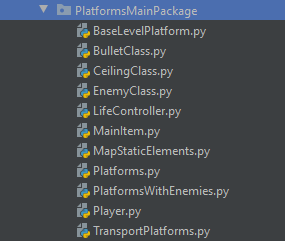
\includegraphics[width=0.5\textwidth]{ProjectStructure/strukturaplatforms.png}
            \caption{Struktura Modułu PlatformsMainPackage}
            \label{StrukturaPlatforms}
        \end{figure}
\newpage

        \item Moduł \textit{PlayFair} (zob. rysunek \ref{StrukturaPlayFair}) zawierający operacje związane z~poziomem kryptograficznym:
        \begin{itemize}
            \item \textit{AnswerField.py} - klasa odpowiadająca za pobieranie odpowiedzi ułożonej przez gracza,
            \item \textit{CheckButton.py} - klasa reprezentująca przycisk sprawdzenia poprawności rozwiązania,
            \item \textit{CopyLetters.py} - klasa odpowiadająca za kopie liter tworzonych przez użytkownika, w~celu rozwiązania zagadki,
            \item \textit{CryptoOperationMain.py} - klasa zawierająca operacje sprawdzające rozwiązanie oraz generowanie klucza szyfrującego,
            \item \textit{LettersPlayFair.py} - klasa odpowiadająca za rysowanie na ekranie liter służących do tworzenia odpowiedzi,
            \item \textit{PlayFairMain.py} - główna klasa poziomu,
        \end{itemize}
        \begin{figure}[hpt!]
            \centering
            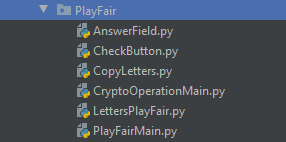
\includegraphics[width=0.5\textwidth]{ProjectStructure/strukturaplayfair.png}
            \caption{Struktura Modułu PlayFair}
            \label{StrukturaPlayFair}
        \end{figure}
    \item \textit{BreakingClass.py} - klasa zawierająca obsługę przerywników w~grze
    \item \textit{DrawBackground.py} - klasa odpowiadająca za wyświetlanie tła dla poziomów
    \item \textit{GameController.py} - klasa zarządzająca rozgrywką
    \item \textit{MainImages.py} - zawiera w~sobie wszystkie wymagane w~grze grafiki
    \item \textit{ResizeClass.py} - zawiera w~sobie funkcje służące do skalowania wyświetlanych obrazków
\end{itemize}
\newpage

\section{Testowanie Gry}
\par Gra \textit{Tree Of Life} została przetestowana za pomocą testów manualnych. Są to testy bazujące głównie na zasobach ludzkich. Jest to czasochłonny proces, ponieważ tester musi sprawdzać każdą funkcjonalność ręcznie. Są one również bardziej podatne na błędy w~porównaniu do testów automatycznych, gdzie proces sprawdzania programu odbywa się za pomocą wcześniej przygotowanych skryptów - scenariuszy.
\par Testerami gry \textit{Tree of Life} byli potencjalni gracze, jak również zawodowi testerzy. Każda osoba po zakończonej rozgrywce odpowiedziała na następujące pytania:
\begin{enumerate}
    \item \textit{Czy podczas grania w~grę TreeOfLife natrafiłeś na jakieś błędy (tzw. bugi)?}
    \item \textit{Czy znalezione błędy przeszkadzały w~rozgrywce?}
    \item \textit{Czy gra jest grywalna?}
    \item \textit{Czy sposób przedstawienia algorytmów w~grze był jasny/zrozumiały?}
\end{enumerate}
\par Podczas testowania testerzy natrafili na różnego rodzaju błędy. Były one głównie związane z~poziomami platformowymi, natomiast poziomy, w~których użytkownik musiał rozwiązać zagadkę algorytmiczną działały bez zarzutów. Większość z~napotkanych błędów dotyczyła generowania przeciwników: nie poruszali się oni po całej dostępnej platformie, jedynie po jej niewielkiej części. Część z~graczy zauważyła również problem z~wykrywaniem kolizji. Jednak te błędy nie przeszkadzały w~rozgrywce.
\par Algorytmy w~produkcji według oceny testerów, przedstawione były w~sposób zrozumiały.


%############################################################################################
%############################################################################################
%-----------            	          Zakończenie                                -----------# 
%############################################################################################
%############################################################################################
\chapter*{Zakończenie}
\addcontentsline{toc}{chapter}{Zakończenie}
\par Pomimo faktu rozpoczęcia pracy w~marcu 2020 roku, gra nie została w~pełni skończona. Jest ona ciągle udoskonalana oraz rozbudowywana o~coraz to nowe elementy. Bazując na doświadczeniu przy tworzeniu gry \textit{Tree Of Life}, która była niekomercyjnym, dwuosobowym projektem, można wyobrazić sobie jak wielki wysyłek muszą włożyć firmy zajmujące się profesjonalnym tworzeniem gier, aby ich tytuły cieszyły się niesłabnącą popularnością. \textit{Tree Of Life} mimo, że nie jest dużą produkcją zawiera w~sobie kilka niedociągnięć - które będą eliminowane, aby przyszli użytkownicy mogli choć w~niewielkim stopniu poznać podstawy świata informatyki, bądź sprawdzić swoją wiedzę na jego temat. Po zakończeniu prac nad grą można stwierdzić, że dwuosobowy zespół to stanowczo za mało na stworzenie rozbudowanej produkcji, która nie będzie miała błędów utrudniających bądź ułatwiających rozgrywkę.

\par W~przyszłości planowane jest przeniesienie gry na silnik \textit{Unity} oraz rozbudowanie jej o~większą liczbę poziomów, a także dodanie wyboru poziomu trudności rozgrywki, tak aby użytkownik mógł wybrać, na jakim stopniu zaawansowania chce grać. 

%###############Bibliografia#####################%

\bibliographystyle{plain}
\bibliography{references}
\listoffigures
\addcontentsline{toc}{chapter}{Spis rysunków}

\end{document}

